\justifying

%%%%%%%%%%%%%%%%%%%%%%%%%%%%%%%%%%%%%%%%%%%%
\section{Introduction}\label{secc3_intro}
%%%%%%%%%%%%%%%%%%%%%%%%%%%%%%%%%%%%%%%%%%%%

\suit~consists of two main sub-units: The \suit~optics package - comprising an off-axis Ritchey-Chr\'{e}tien telescope, and \suit~Electronics package - responsible for communicating with the telescope to perform imaging. The main components of the \textit{SUIT} optics package include a multi-operation entrance door, a thermal filter to control the amount of incoming sunlight, primary and secondary mirrors, a shutter mechanism to control exposure times, baffles to reduce stray and scattered light, a motorized filter wheel assembly, a piezoelectric focusing mechanism, and a CCD detector. Figure \ref{fig:suit} shows a schematic diagram of the telescope.

%%%%%%%%%%%%%%%%%%
\begin{figure}
    \centering
    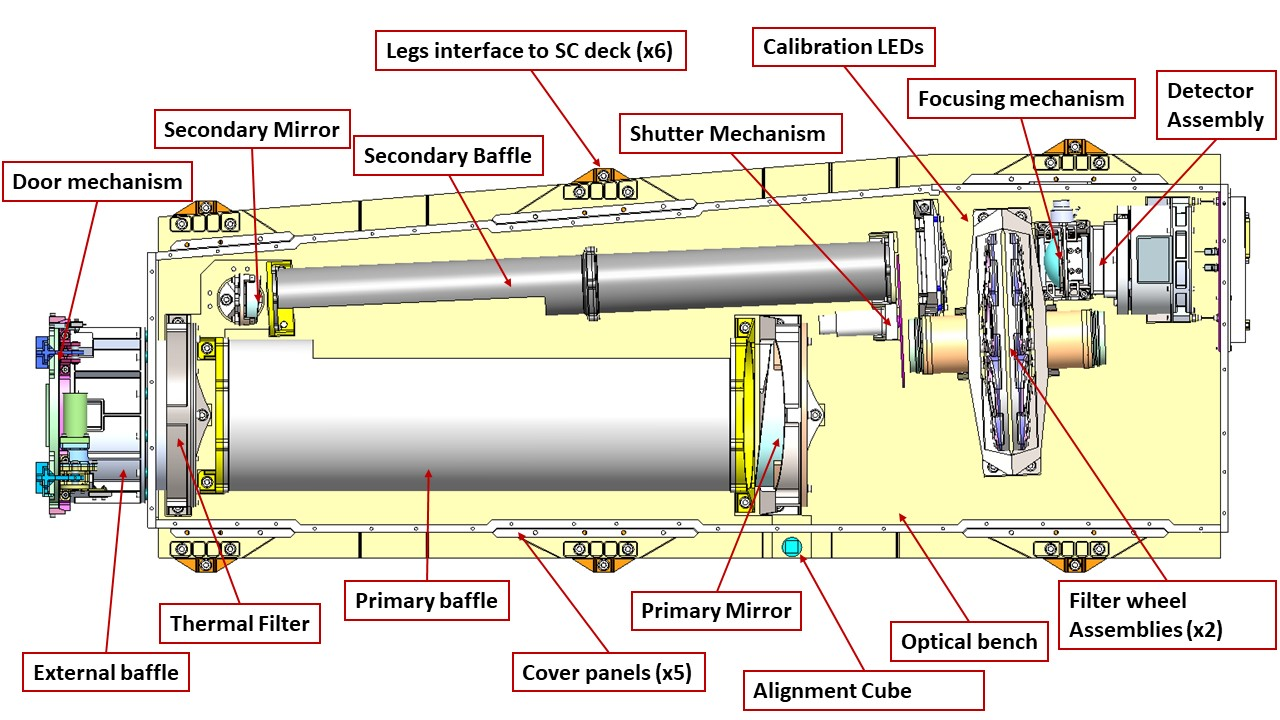
\includegraphics[width=0.8\textwidth]{SUITLayout.jpg}
    \caption{Schematic diagram of the \textit{SUIT} telescope.}
    \label{fig:suit}
\end{figure}
%%%%%%%%%%%%%%%%%%

\suit~observes the Sun in eleven spectral bands, of which three are broadband (referred to as BB) and eight are narrow bands (referred to as NB), as listed in Table~\ref{tab:science_filters}. These are used to image different heights of the solar atmosphere, from the photosphere to the chromosphere. In the wavelength range of interest, i.e., 200--400 nm, the solar flux increases by two orders of magnitude (see Fig.~\ref{fig:sun_spec}). The spectrum is SOLSTICE and SOLSPEC solar flux combined. Therefore, we must employ certain combination filters to control solar flux levels and achieve the best signal-to-noise ratio (SNR) at each filter bandpass. These combination filters are listed in the second column of Table~\ref{tab:science_filters}. Note that \textit{SUIT} uses BB01 as a combination filter for NB01 and BB01. Similarly, NB08 is used as a combination filter for another NB08 filter. In total, \textit{SUIT} has 16 filters mounted on two filter wheels, each having eight slots. A given filter combination is achieved by rotating the two filter wheels independently and placing the desired filter combination in the beam path.

%------------------------------------------------------------
\begin{figure}
    \begin{center}
    \begin{tabular}{c}
    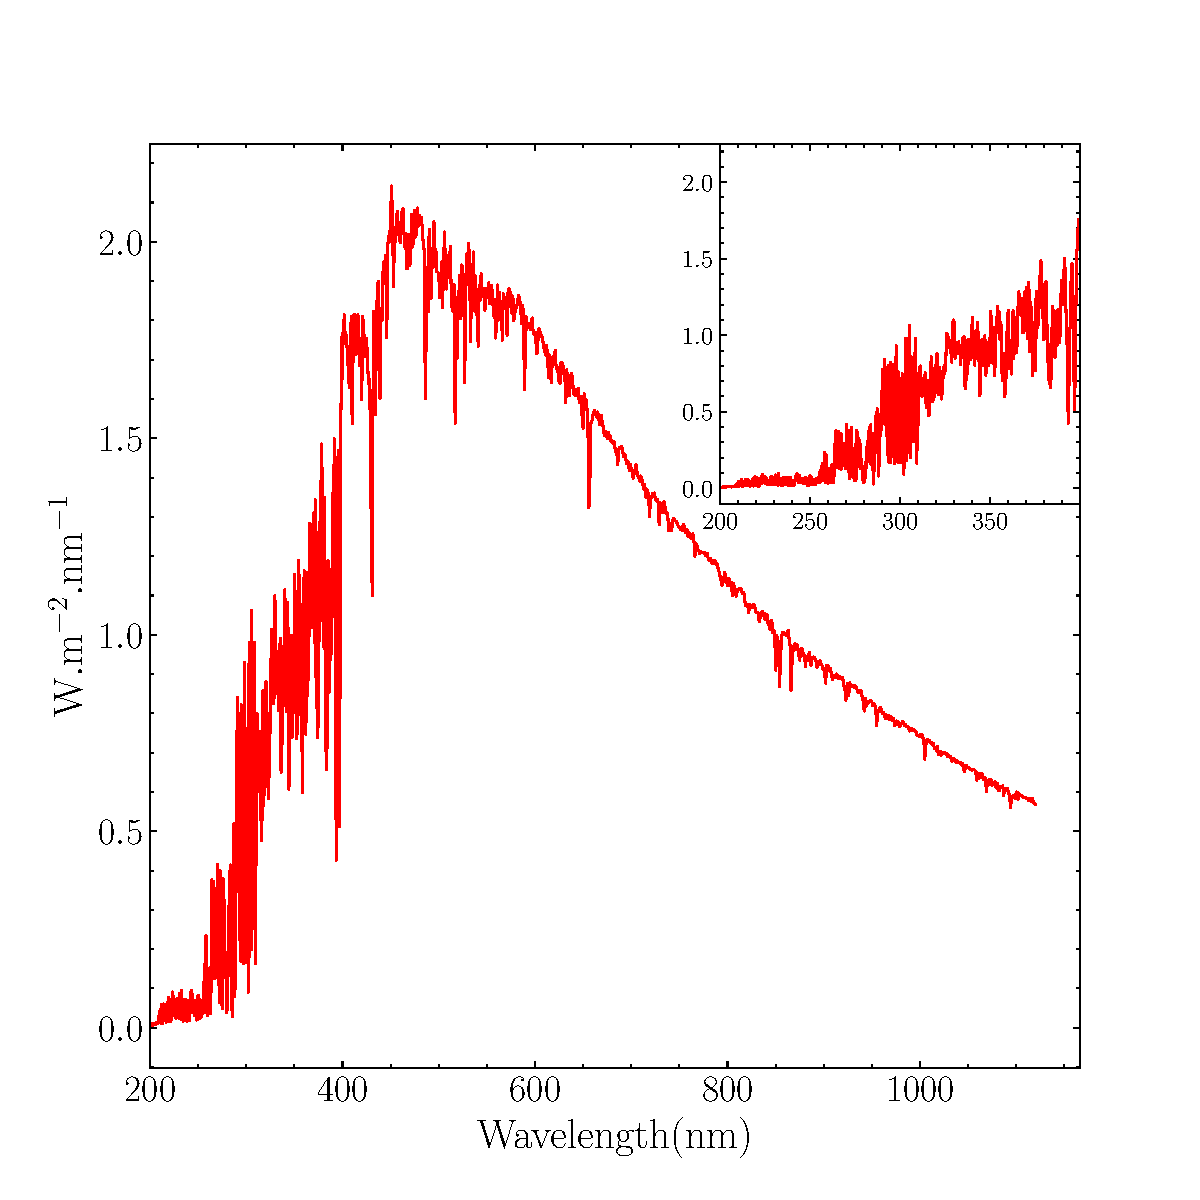
\includegraphics[trim={0.8cm 0cm 2cm 1.2cm},clip,width=0.6\linewidth]{solar_spec_2.pdf}
    \end{tabular}
    \end{center}
\caption{The solar spectrum from SOLSTICE and SOLSPEC combined. The inset plot shows a dramatic rise in solar irradiance within \suit's observation band.} 
\label{fig:sun_spec} 
\end{figure} 
%-----------------------------------------------------------


%-----------------------------------------------------------
\begin{table*}[ht!]
\begin{center}
\begin{tabular}{||l|c|c|c|r||}
\hline
\textbf{Science}  &	\textbf{Combination} &	\textbf{Central} & \textbf{Bandpass} &\textbf{Science} \\
\textbf{Filter}	&	\textbf{Filter}     &	\textbf{Wavelength  (nm)}	&		\textbf{(nm)	}	   	&\textbf{target}		\\
\hline
NB1     & BB1 		& 214.0 		    & 11.0 		& Continuum\\
NB2 	& BP2		& 276.7				& 0.4 		& Mg~\rm{II}~k blue wing \\
NB3 	& BP2		& 279.6 			& 0.4 		& Mg~\rm{II}~k\\
NB4 	& BP2		& 280.3				& 0.4 		& Mg~\rm{II}~h\\
NB5		& BP2		& 283.2				& 0.4 		& Mg~\rm{II}~h red wing\\
NB6 	& BP3		& 300.0 			&1.0 		& Continuum\\
NB7 	& BP3		& 388.0				&1.0 		& CN Band\\
NB8		& NB8		& 396.85 			& 0.1 		& Ca~\rm{II}~h\\
BB1 	& BB1		& 220.0				& 40.0		& Herzberg Continuum \\
BB2 	& BP4		& 277.0 			& 58.0       & Hartley Band\\
BB3 	& BP4		& 340.0				& 40.0        & Huggins Band\\
\hline
\end{tabular}
\end{center}
\caption{List of science filters on board \suit. Columns from left to right denote filter mnemonics (including science and combination filters; NB: Narrowband, BB: Broadband, BP: Bandpass), central wavelengths for science filters and corresponding bandpasses, and the observation interest for the filter.} 
\label{tab:science_filters}
\end{table*}
%-----------------------------------------------------------






%%%%%%%%%%%%%%%%%%%%%%%%%%%%%%%%%%%%%%%%%%%%
\section{Analysis of Spacecraft jitter simulation for {\suit}}\label{sec:suit_jitter}
%%%%%%%%%%%%%%%%%%%%%%%%%%%%%%%%%%%%%%%%%%%%

One of the key steps in estimating the imaging performance was to quantify, if the RMS level of spacecraft jitter would affect the imaging across various exposure time. For this purpose we analyzed the simulated spacecraft drift data provided by the ISRO URSC team to quantify the RMS jitter as a function of exposure time. There are two main moving components within the payload that can generate significant jitter on the payload, namely the shutter door and the filter wheel (FW) movement. The payload has a FW movement torque compensator in place, to minimize the jitter generated by the FW movement. So, there were four main scenarios that were simulated to be analyzed arranged from least to most amount of jitter:

%%%
\begin{enumerate}
    \item No shutter torque + no filter movement
    \item Only shutter torque
    \item Shutter torque + FW movement + FW compensation torque
    \item Shutter torque + FW movement + no FW compensation torque
\end{enumerate}
%%%

%%%%%%%%
\begin{figure}
    \centering
    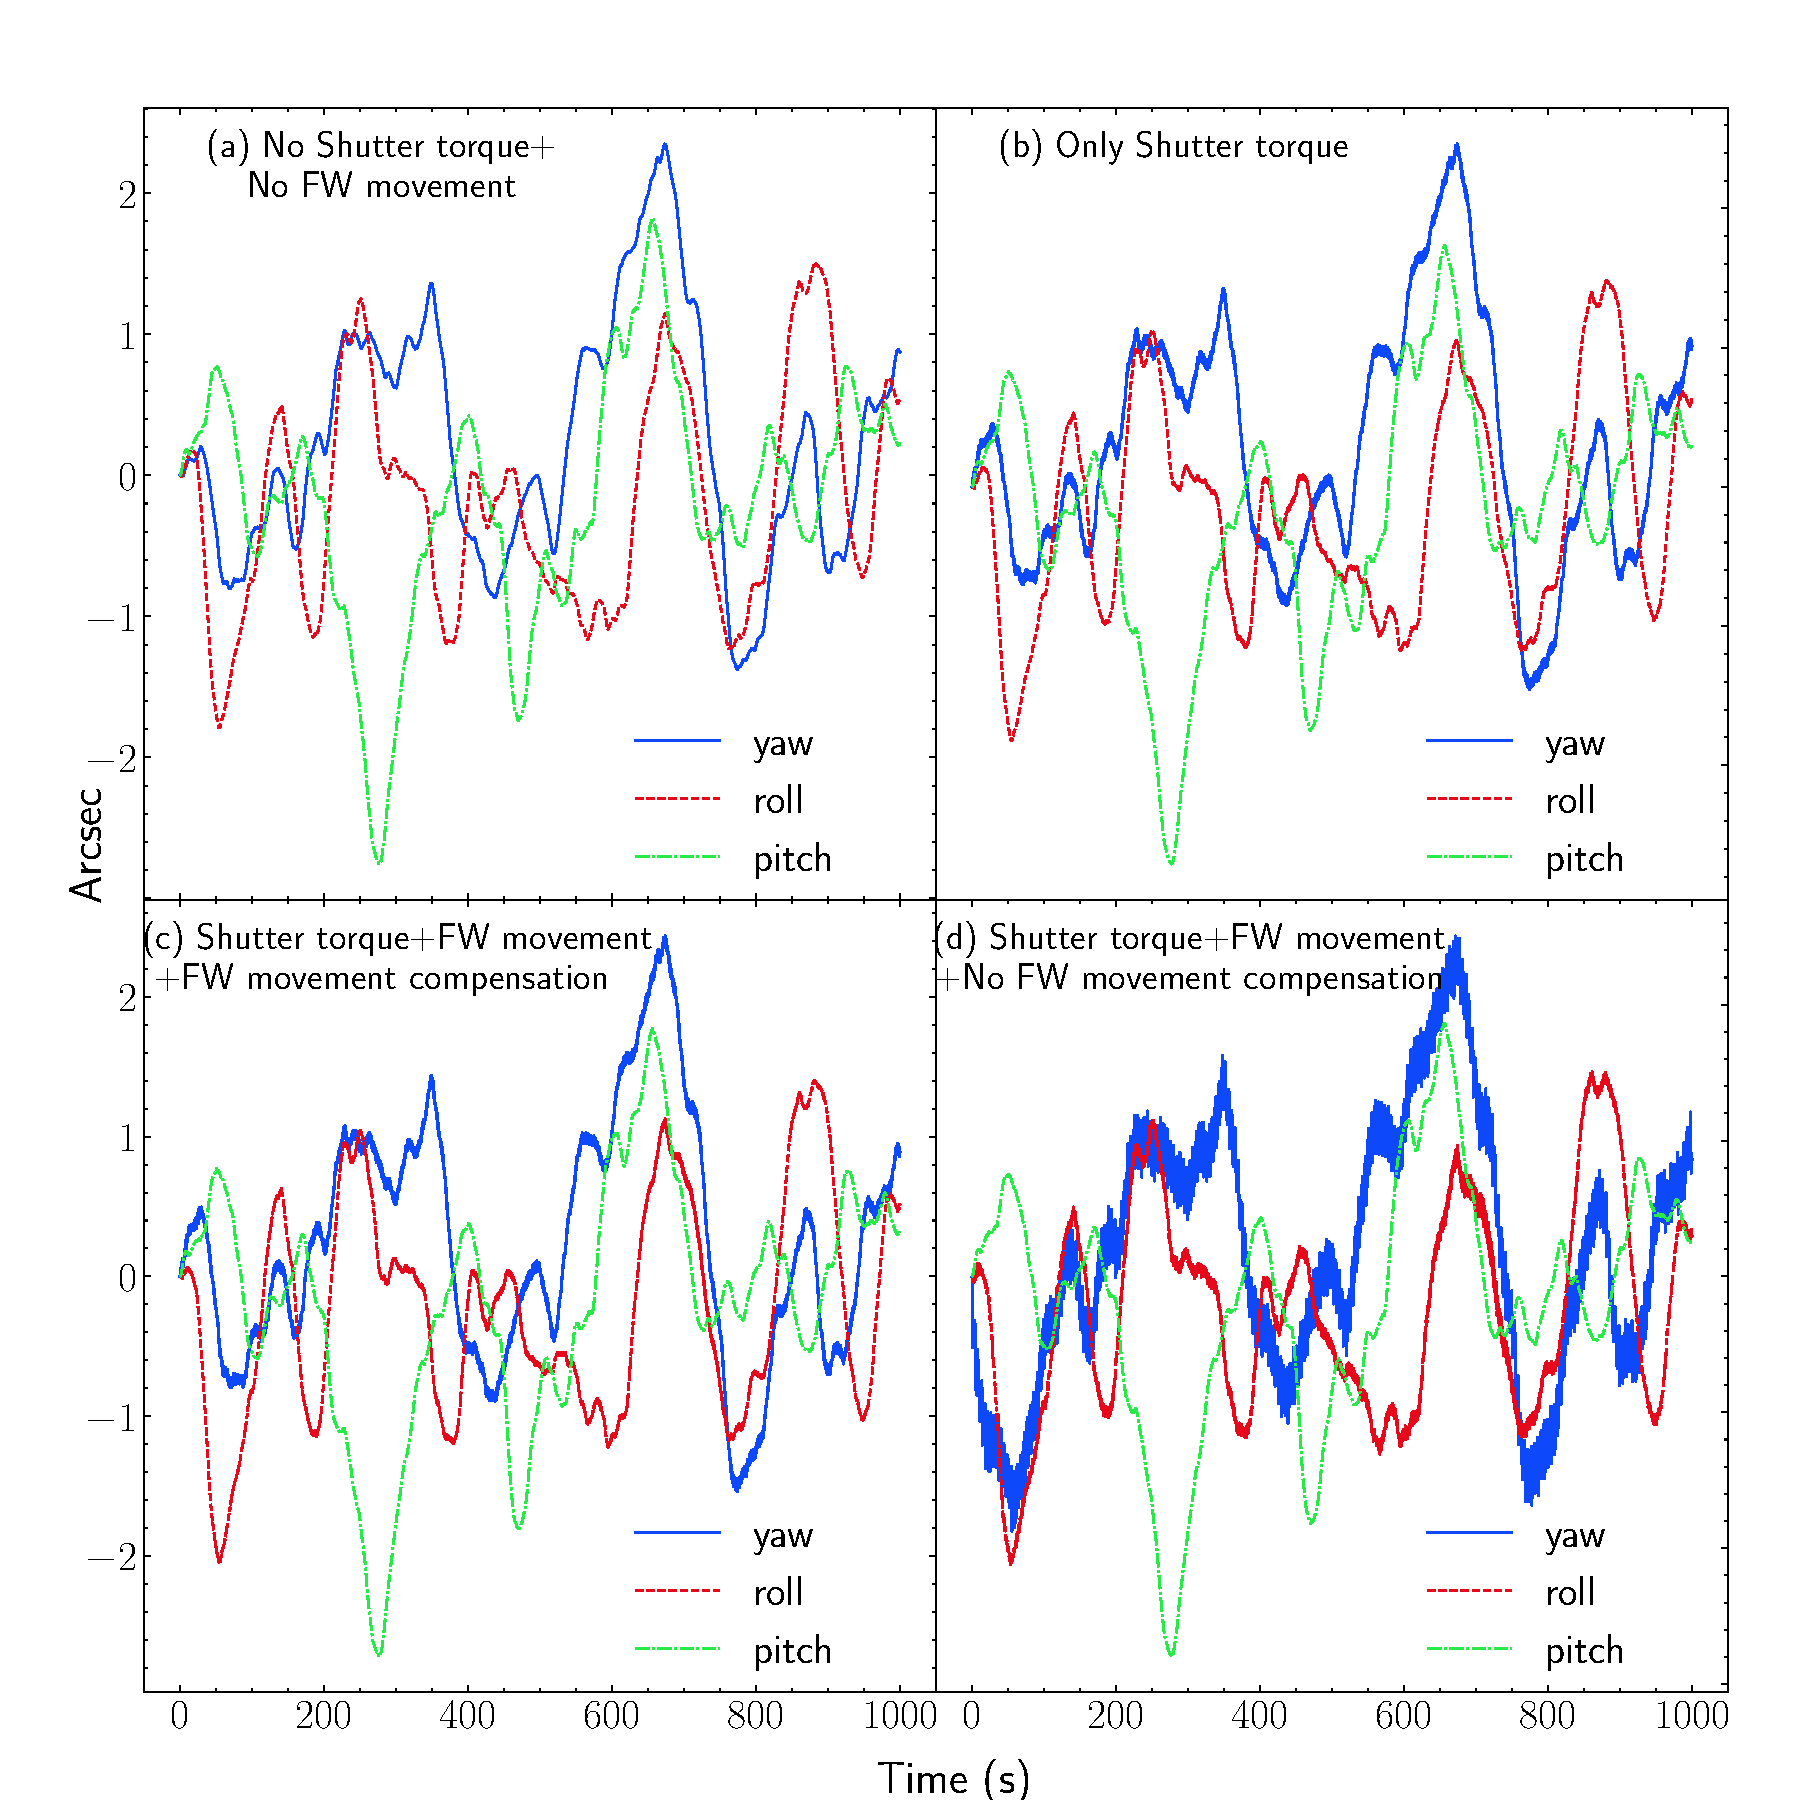
\includegraphics[trim={1cm 0cm 1cm 1cm},clip,width=0.7\textwidth]{jitter_sim.pdf}
    \caption{The figure shows the simulated drift for the yaw, roll and pitch axis of the payload as a function of time for the aforementioned four cases in \S\ref{sec:suit_jitter}. The panel (a) shows the simulated drift when there is no shutter or FW movement. Panel (b) shows the same when there is only shutter movement. Panel (c): when there is both shutter and FW movement and FW movement compensation is employed. Panel (d): when there is both shutter and FW movement but the FW movement compensation is not employed.}
    \label{fig:jitter_sim}
\end{figure}
%%%%%%%%

The Fig.~\ref{fig:jitter_sim} shows the simulated drift for the aforementioned four cases. We did a Fourier analysis of the simulated drift data to characterize the spacecraft jitter from the spacecraft drift. The Fig.~\ref{fig:jitter_sim_ps} shows the power spectrum for the simulated drift shown in Fig.~\ref{fig:jitter_sim}. The SUIT imaging channels have a maximum possible exposure$~\sim$~1.4 s, which corresponds to a frequency of~$\sim$~0.7 Hz and lower exposures would correspond to a higher frequency. So, signals in the Fourier transform corresponding to 0.7 Hz or higher are capable of affecting the imaging within the exposure window. We assumed any signal with a frequency 0.5 Hz or greater from the Fourier transform to be Jitter signal. We then took a frequency cut at 0.5 Hz, of the power spectrum to filter the drift from the jitter and then took an inverse FT to reconstruct the jitter signal for the three axis. To calculate the amount of RMS jitter on various time scales relevant in the context of SUIT exposure times, we took the extracted jitter signal and picked out bins of multiple time scales and calculated the RMS jitter for them. We had several bins for each time scale, each of which gave us RMS jitter and maximum jitter within that bin. We averaged all the bins to estimate the RMS jitter and maximum Jitter for that specific timescale. Figures \ref{fig:rms_jitter} ad \ref{fig:max_jitter} shows the RMS and maximum jitter as a function of timescale. SUIT has a 0.7\arcsec/pix resolution. Both the average and the maximum jitter even in the worst case scenario, i.e when shutter torque and FW movement is present but the FW movement compensation is not employed, is much lower than the pixel size of SUIT within timescales relevant to exposure times for SUIT. We did not need to account for the jitter while characterizing the imaging performance.

%%-----------------------------%%
\begin{figure}
    \centering
    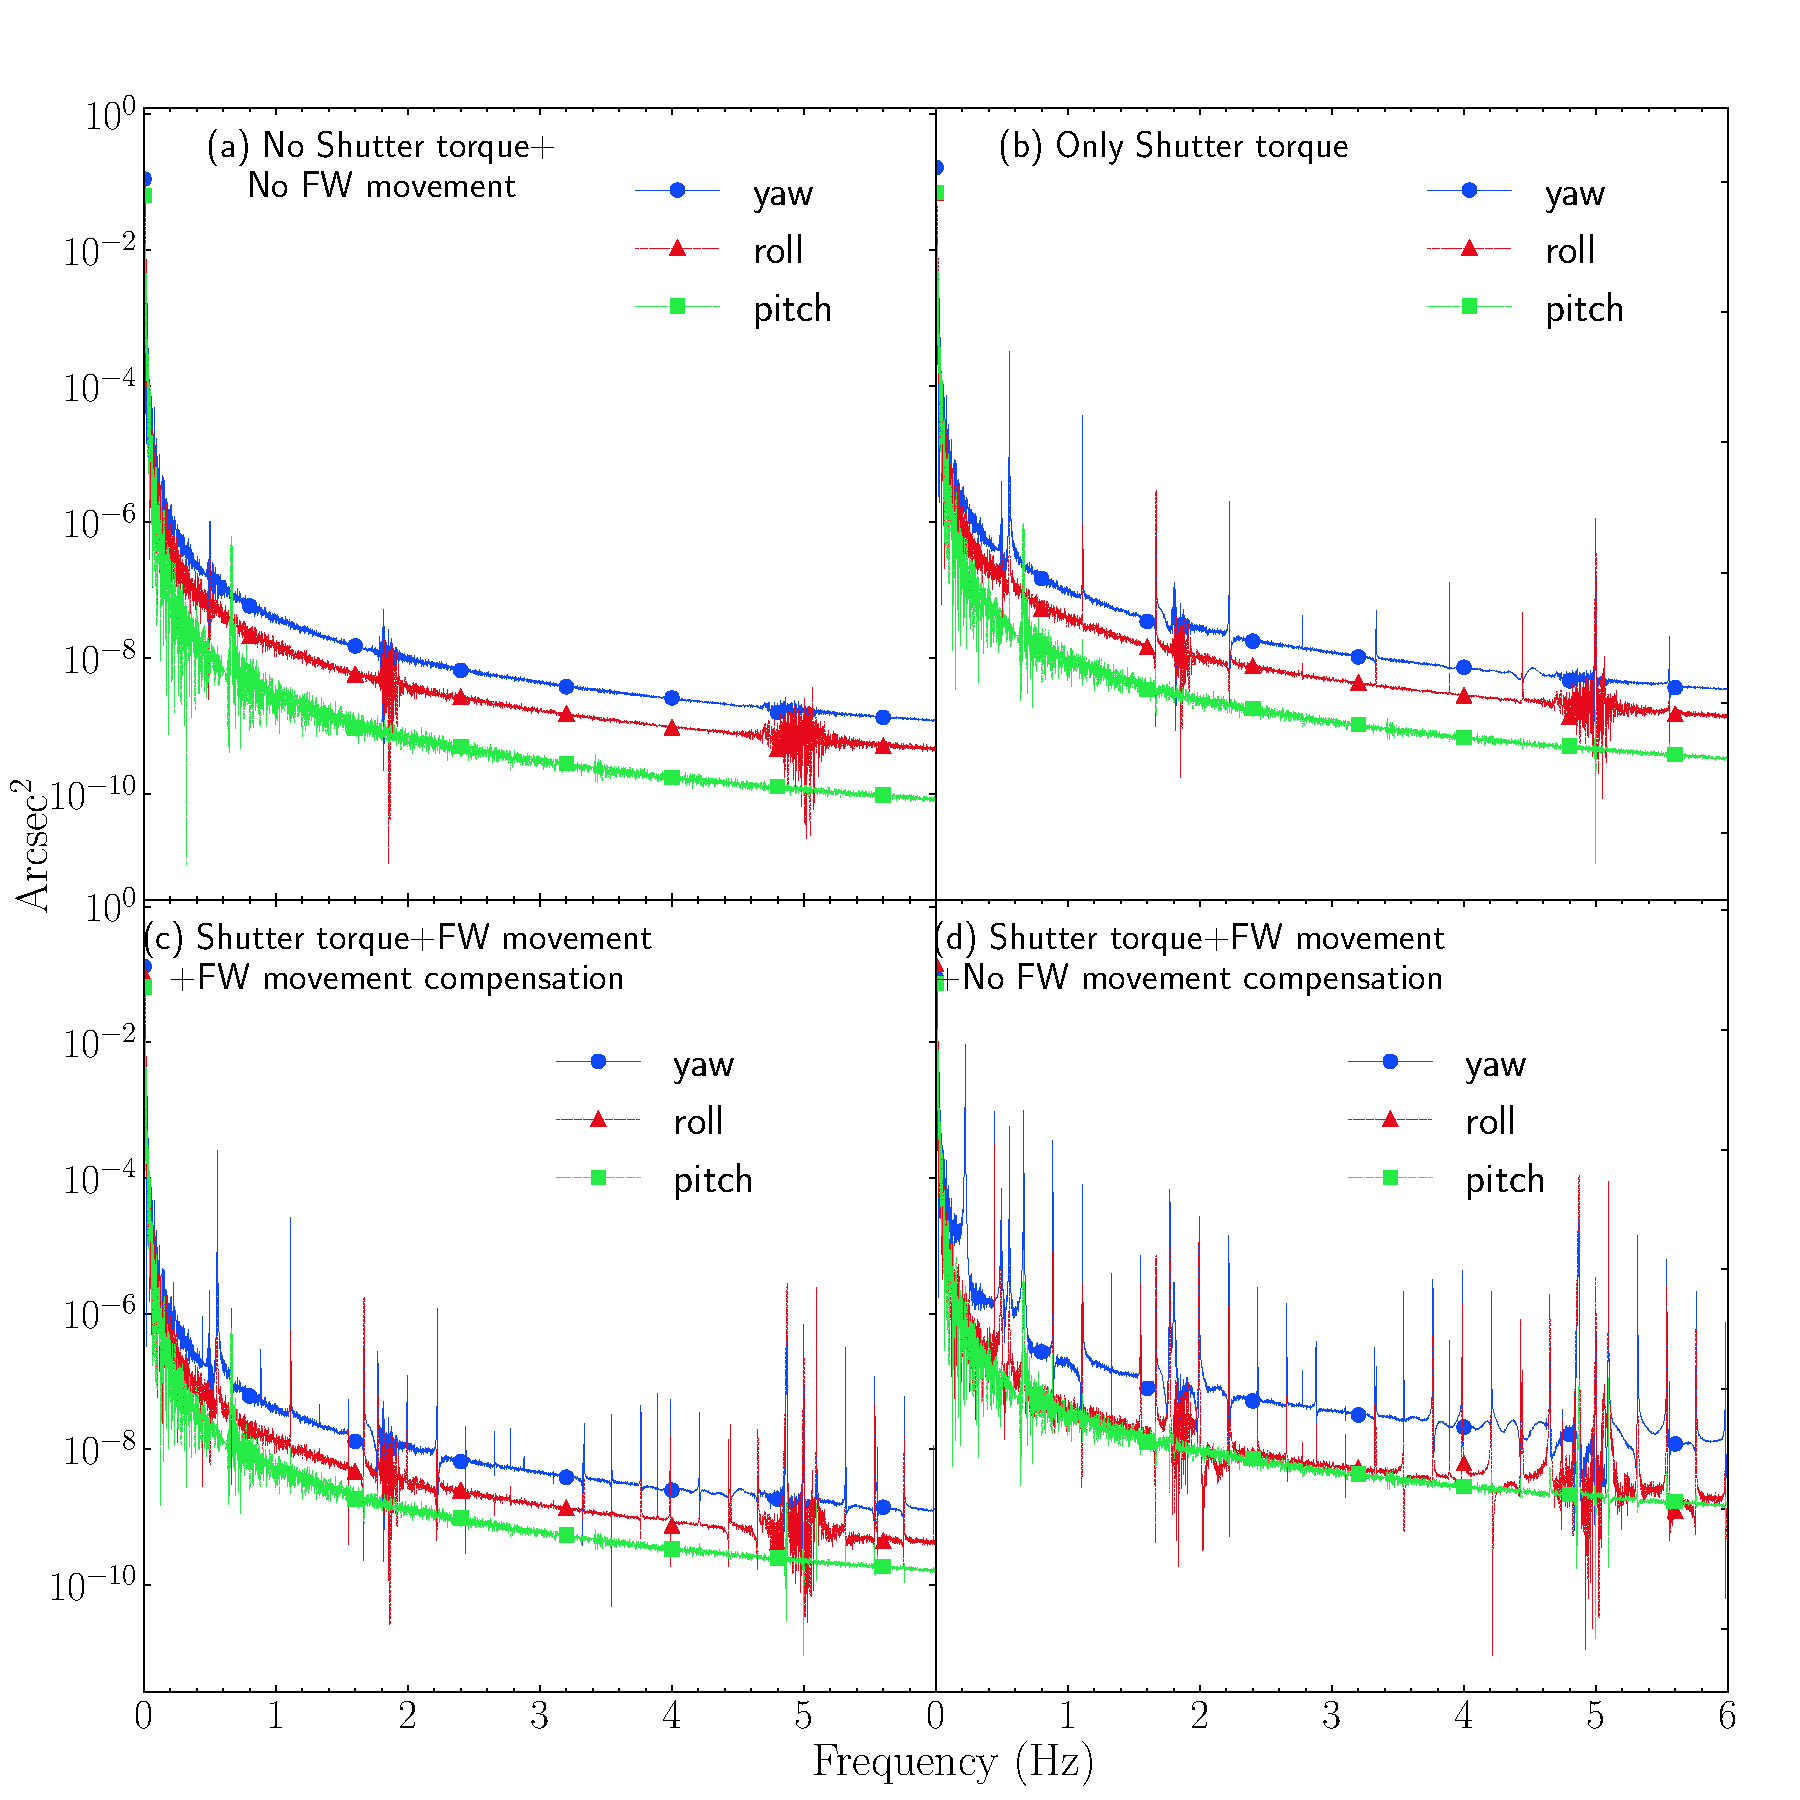
\includegraphics[trim={0cm 0cm 1cm 1cm},clip,width=0.7\textwidth]{jitter_psd.pdf}
    \caption{The figure shows the FT of the simulated drift for the yaw, roll and pitch axis of the payload as a function of time for the aforementioned four cases in \S\ref{sec:suit_jitter}. The \textbf{panel (a)} shows the FT of the simulated drift when there is no shutter or FW movement. \textbf{Panel (b)} shows the same when there is only shutter movement, \textbf{panel (c)}: when there is both shutter and FW movement and FW movement compensation is employed, \textbf{panel (d)}: when there is both shutter and FW movement but the FW movement compensation is not employed.}
    \label{fig:jitter_sim_ps}
\end{figure}
%%-----------------------------%%

%%-----------------------------%%
\begin{figure}
    \centering
    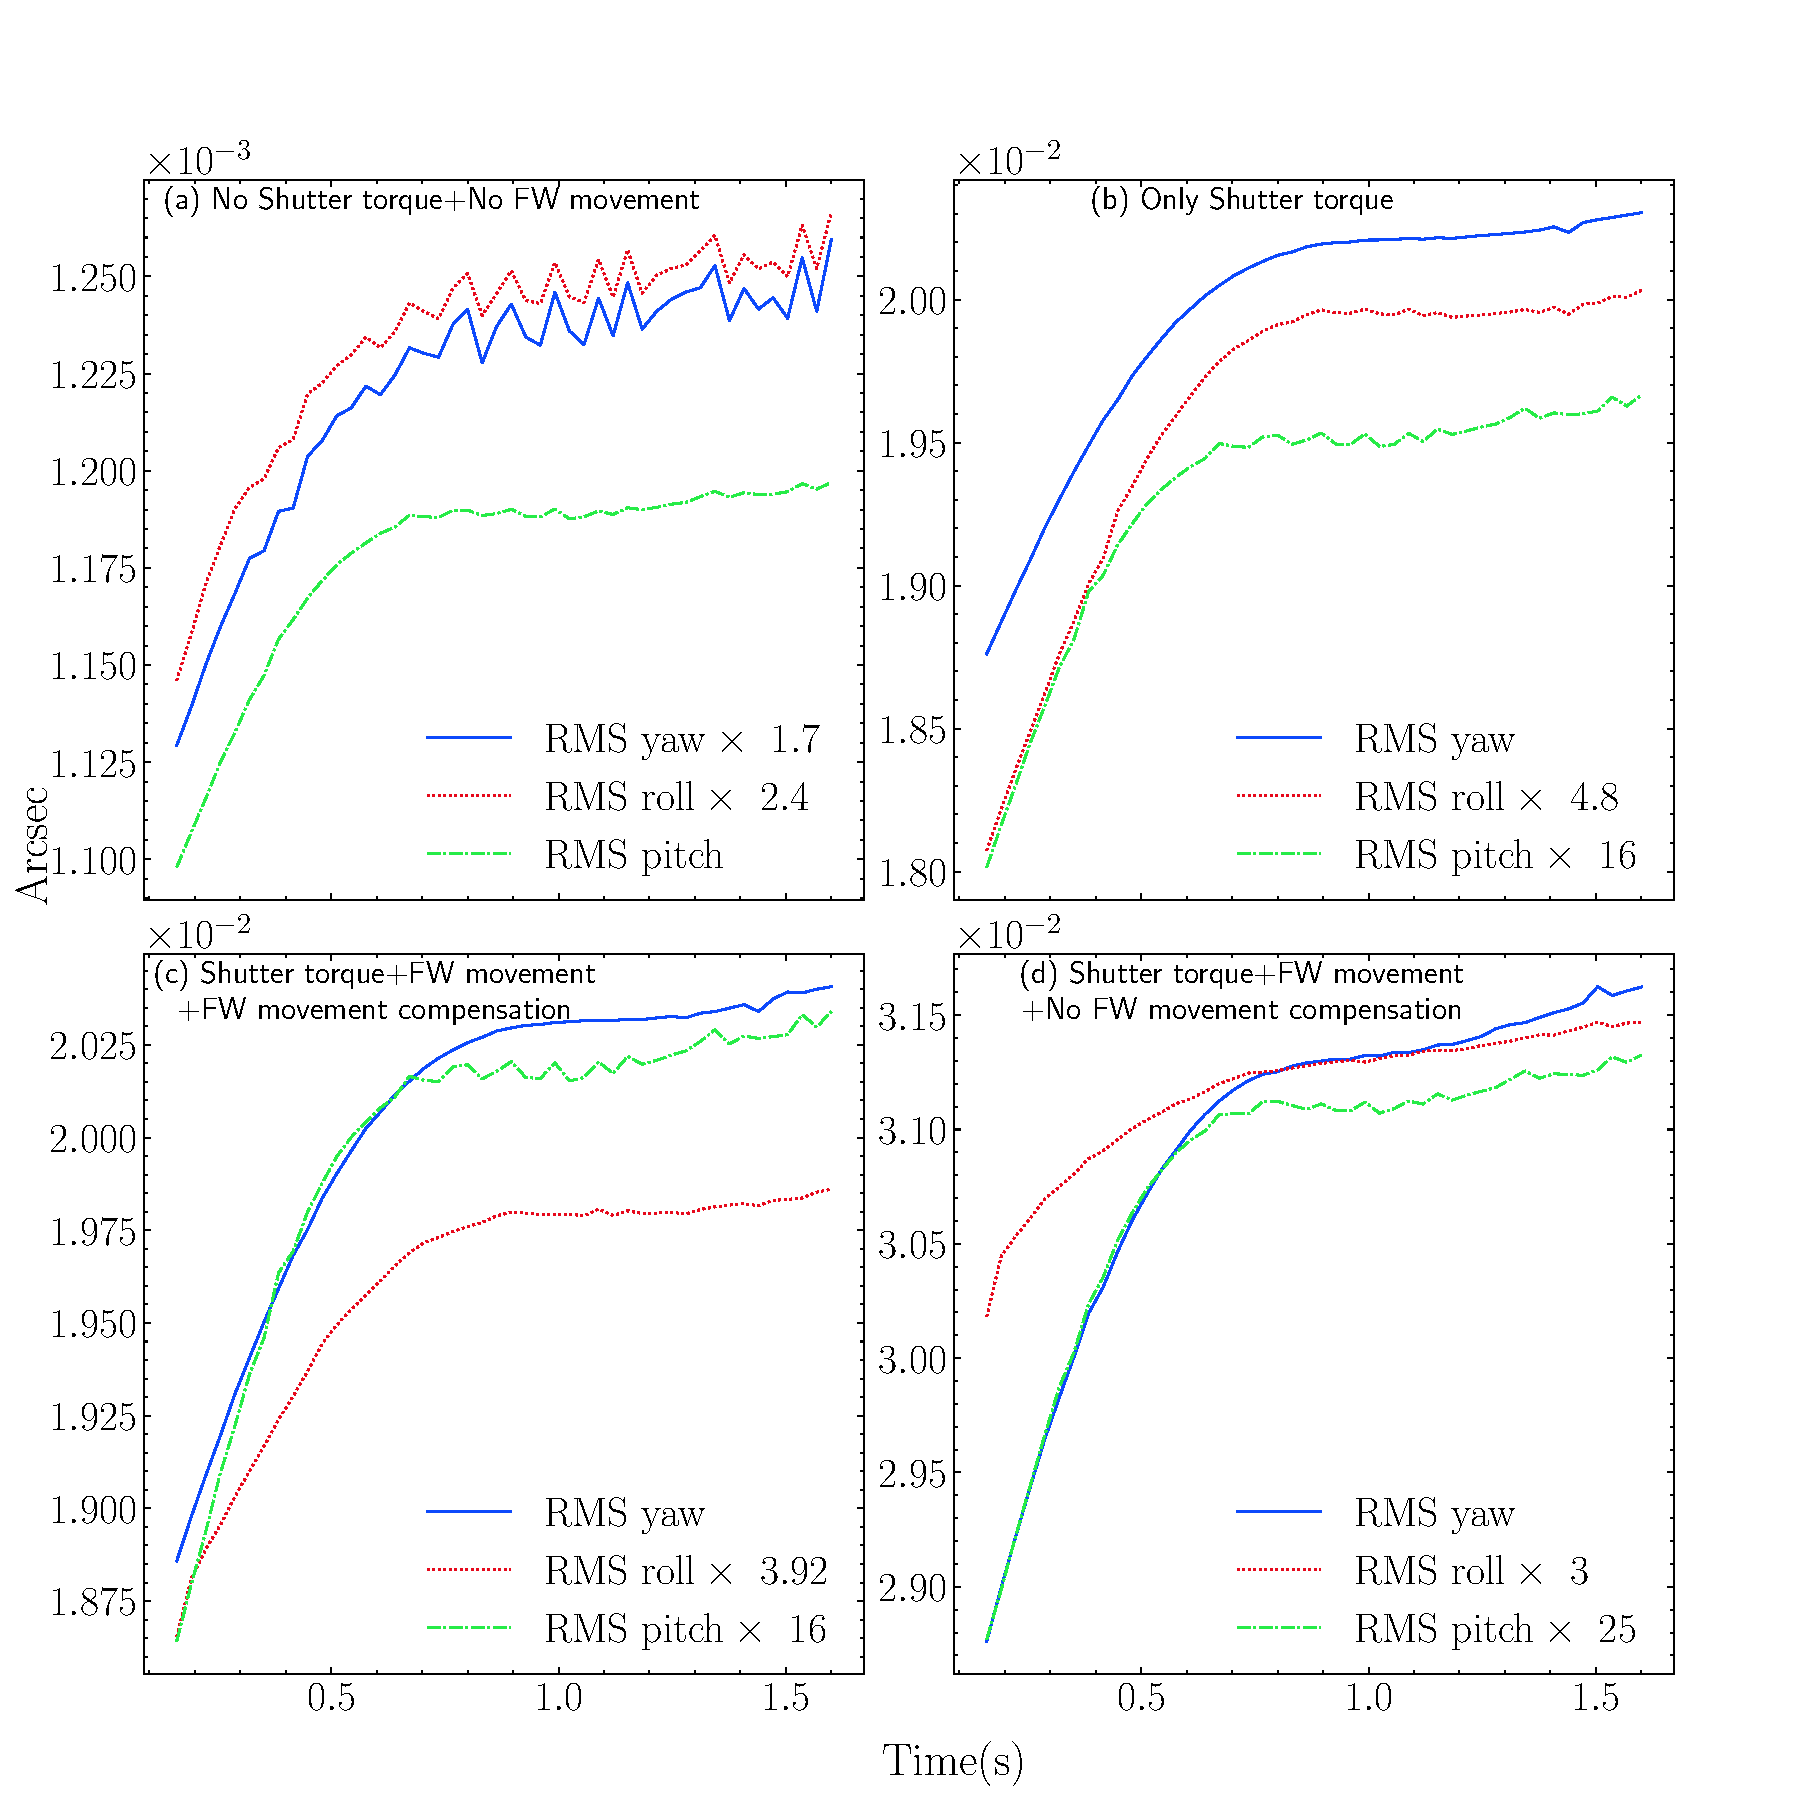
\includegraphics[trim={0cm 0cm 1cm 1cm},clip,width=0.7\textwidth]{rms_jitter.pdf}
    \caption{The RMS jitter at various timescales for the four scenarios of operation.}
    \label{fig:rms_jitter}
\end{figure}
%%-----------------------------%%

%%-----------------------------%%
\begin{figure}
    \centering
    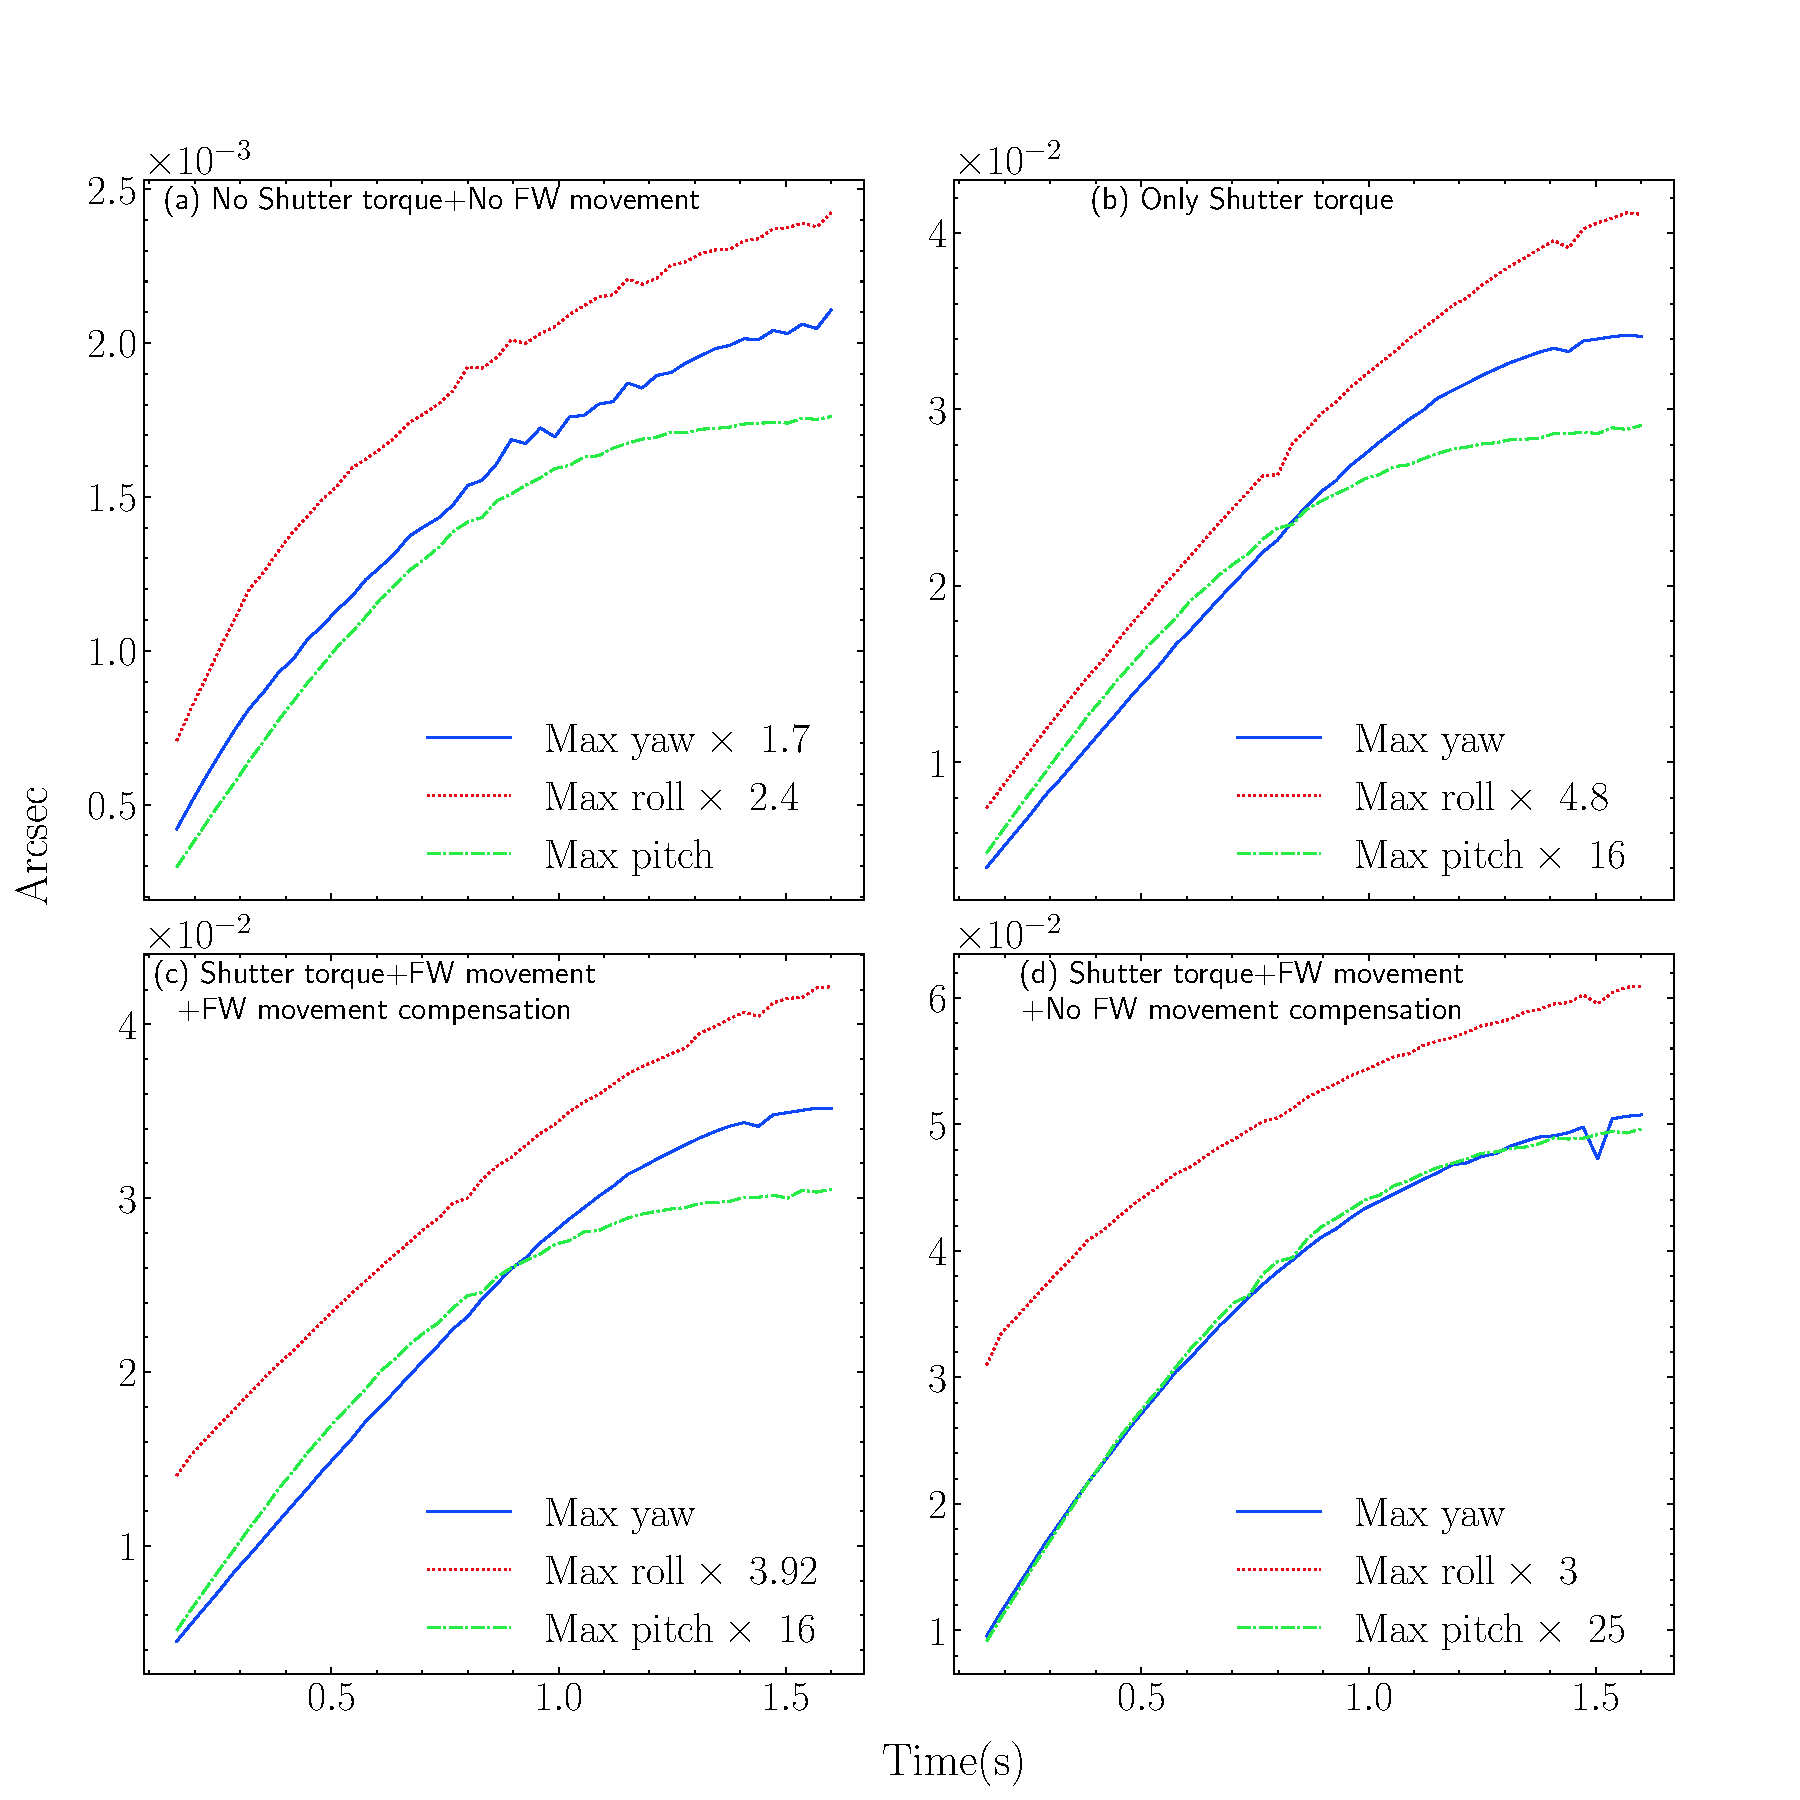
\includegraphics[trim={0cm 0cm 1cm 1cm},clip,width=0.7\textwidth]{max_jitter.pdf}
    \caption{The Maximum jitter at various timescales for the four scenarios of operation.}
    \label{fig:max_jitter}
\end{figure}
%%-----------------------------%%

%%%%%%%%%%%%%%%%%%%%%%%%%%%%%%%%%%%%%%%%%%%%
\section{Throughput model of {\suit}}\label{sec:suit_throughput}
%%%%%%%%%%%%%%%%%%%%%%%%%%%%%%%%%%%%%%%%%%%%

The design of the \suit~telescope prioritizes throughput and photometric accuracy requirements. Optical parameters of various optical elements, such as the reflectivity of primary and secondary mirrors, transmission of the thermal filter, field corrector lens, spectral transmission of the science filter, and combination filter, are optimized to maximize throughput within their corresponding wavelength ranges.

The optical response of \suit~is evaluated based on the solar spectral irradiance and the throughput characteristics of each sub-assembly. Experimental throughput data is compared with a throughput model to validate the consistency between experimental and simulated results. This validation process is crucial for determining exposure times for the payload across the eleven science bandpasses in different operational modes.

The throughput of \suit~is modeled using the Sun-as-a-Star spectrum to predict counts for specific science filter combinations. The measured wavelength responses of individual components are utilized to estimate these counts. If the photon flux incident at the entrance aperture is denoted by $P(\lambda)$, then the recorded data number in the images can be expressed as:

%%%%%%%%%
 \begin{equation}\label{eq1}
     DN~=~\int~P(\lambda)~R(\lambda)~t~d\lambda
 \end{equation}
 %%%%%%%%%
where $R(\lambda)$ is the effective area for the specific science filter combination, and $t$ is the exposure time for that filter. The effective area $R(\lambda)$ is derived by multiplying the measured response of all the optical sub-assemblies in the beam path-

%%%%%%%%%
\begin{equation}
    R(\lambda)~=~TF(\lambda)\times PM(\lambda)\times SM(\lambda)\times SF_{i}(\lambda)\times SF_{j}(\lambda)\times L(\lambda)\times QE(\lambda)\times A
    \label{eq:eff_area}
\end{equation}
%%%%%%%%%
where $TF(\lambda), PM(\lambda), SM(\lambda), SF_{i}(\lambda), SF_{j}(\lambda), L(\lambda)~and~QE(\lambda)$ are the measured responses as a function of wavelength of thermal filter, primary mirror, secondary mirror, filters in filter wheel 1 and 2, field corrector lens and the quantum efficiency of the CCD. The effective area curves for each filter are shown in Fig.~\ref{fig:eff_area}.

%%%%%%%%%%%
\begin{figure}
    \centering
    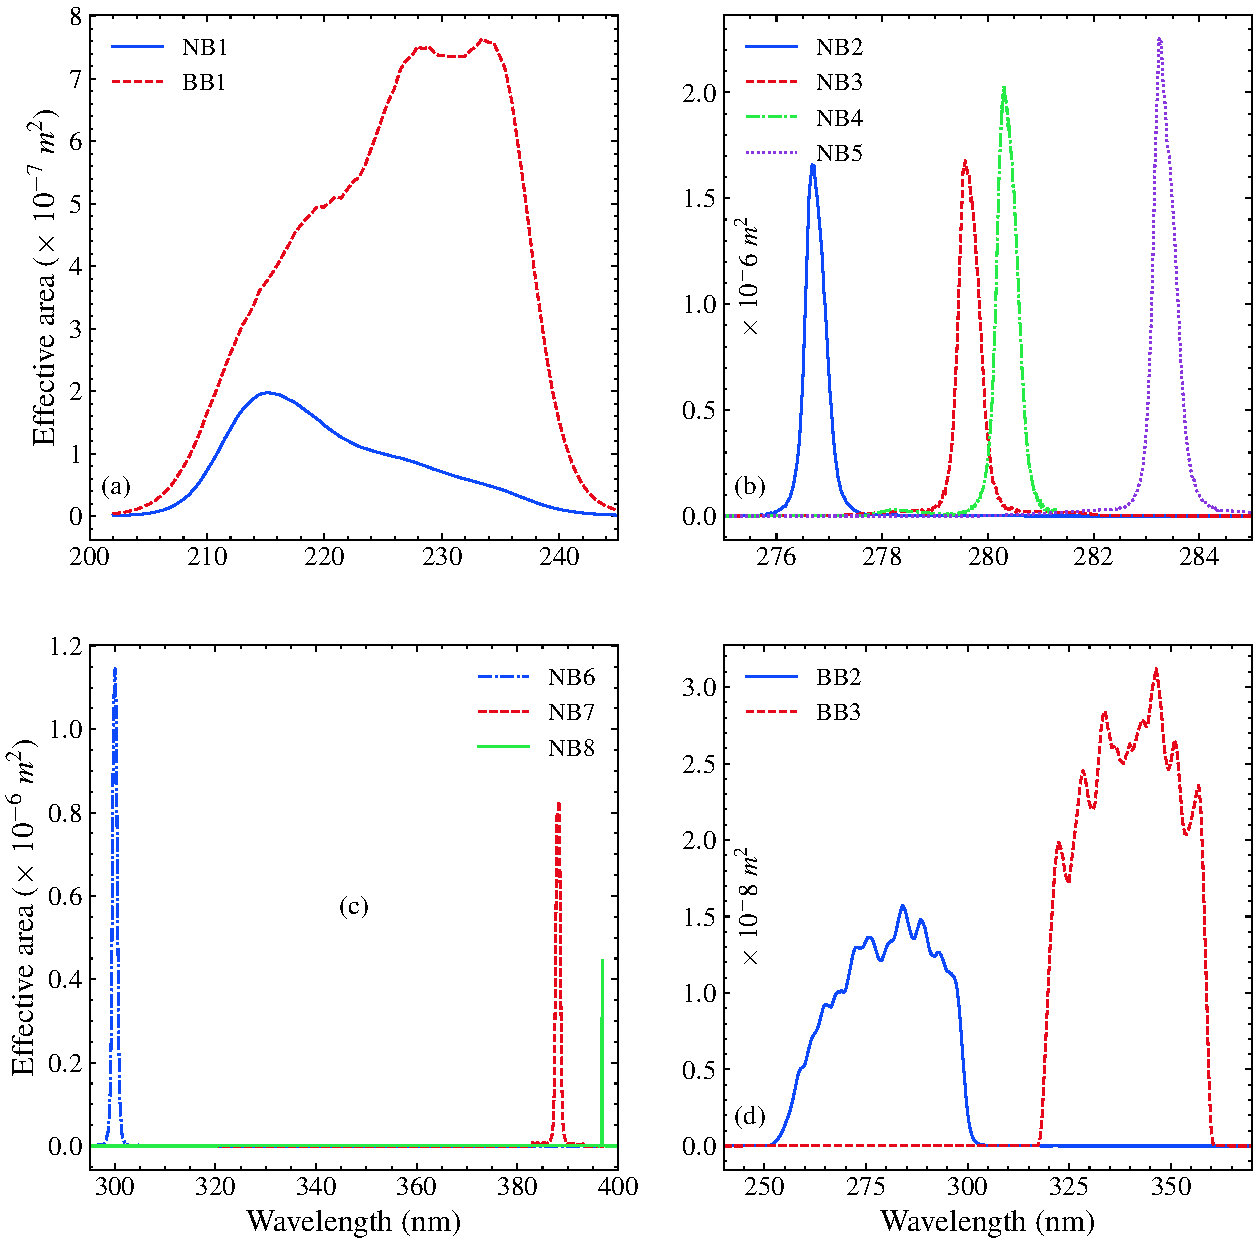
\includegraphics[width=0.7\textwidth]{eff_area.pdf}
    \caption{The effective area curves for SUIT science filters.}
    \label{fig:eff_area}
\end{figure}
%%%%%%%%%%%

%%%%%%%%%%%%%%%%%%%%%%%%%%%%%%%%%%%%%%%%%%%%
\section{Photometric Calibration and Spectral Validation {\suit}}\label{sec:suit_radiometric}
%%%%%%%%%%%%%%%%%%%%%%%%%%%%%%%%%%%%%%%%%%%%

To achieve the scientific goals, photometric and spectral calibration of the payload is of utmost importance. The photometric throughput of the telescope is modeled during instrument design to ensure the required photometric throughput accuracy of 1\%. For this purpose, Light of a known wavelength and measured intensity is fed into the payload from a monochromator after collimation. The payload is operated in a vacuum chamber to simulate space-like conditions in this setup. For the details of the experimental setup refer to \cite{sarkar24}. We use these measurements and compare them with our throughput model to validate the measurements of the transmission profiles. We also use these measurements to validate the spectral transmission profile of the science filter channels.

%%%%%%%%%%%%%%%%%%%%%%%%%%%%%%%%%%%%%%%%%%%%%%%%%%%%%%%%%%
\subsection{Photometric Calibration}\label{sec:calibration}
%%%%%%%%%%%%%%%%%%%%%%%%%%%%%%%%%%%%%%%%%%%%%%%%%%%%%%%%%%

In this test, an optical fiber is used to feed light from the monochromator at the focal plane of the SUIT collimator. The monochromator uses a grating with a density of 1200 lines per mm (lpmm) and a nominal dispersion of 1.44 nm/mm, blazed at 500 nm. The spectral resolution of the monochromator depends on the entrance slit or the exit slit, whichever is geometrically wider. In our case, an entrance slit width of 3 mm is used to maximize the light output from the spectrograph. The emergent monochromatic light has a wavelength band of \(3 \times 1.44 = 4.32\) nm. This wavelength band accommodates the complete transmission spectrum of all the narrow band science filters being tested. The fiber carries light from the monochromator, which is collimated and fed into~\suit.

A UV-enhanced photo diode, certified by the National Institute of Science and Technology (NIST) as traceable (specifically the Newport 918D-UV-OD3R model), is used to quantify the net output flux of the collimator. Both the monochromator and photo diode are set to align with the wavelength corresponding to the science filter under test. It's noteworthy that the Xenon lamp's spectral intensity remains stable within a 4.32 nm band, exhibiting a flat profile. By dividing the measured photo diode's output flux(\(nWm^{-2}\)), by the wavelength band of the spectrograph, we derive the spectral flux from the collimator(\(Wm^{-2}nm^{-1}\)). Following this, the photo diode is removed from the beam path, and an image of the fiber bundle is captured using \suit. The fiber face is obscured to record the background value, and another exposure is initiated. These findings are directly comparable with the modeled throughput derived from the Sun-as-a-Star spectrum for various filter wavelength bands. The following steps are followed to do that:

\begin{itemize}
     \item The background count is estimated by taking the median of the fiber occulted image.
     \item From the background corrected optical fiber images, we calculate the 99\% ensquared energy radius and the total enclosed data counts ($DN_{0.99}$).
     \item The photo diode gives the measurement of corresponding input flux ($E_{0.99}$) in units of $nW.m^{-2}$ for an input spectral bin of 4.32 nm. The flux is divided by the spectral bin size to get the spectral irradiance per unit area in units of $nW.m^{-2}.nm^{-1}$. The ratio of $DN_{0.99}$ and ${E_{0.99}}$ tells the expected counts for any given input flux, $F~=~\nicefrac{DN_{0.99}}{E_{0.99}}$ in units of $DN.s^{-1}/(nW.m^{-2}.nm^{-1})$ for that science filter bandpass.
     \item We use a composite SOLar STellar Irradiance Comparison Experiment (SOLSTICE; 115{--}320 nm) onboard the SOlar Radiation and Climate Experiment (SORCE) \cite{rottman05,harder05,mcclintock05} satellite and SOLar SPECtrometer (SOLSPEC) \cite{thuillier09} solar spectrum as our standard for solar radiation. Using the spectra, we can calculate the total energy input from the Sun for the concerned filter within the wavelength extent, $E_{\odot}~=~\int_{\lambda_{1}}^{\lambda_{2}}~P(\lambda)~d\lambda$, where $P(\lambda)$ is the SOLSTICE, SOLSPEC composite solar spectrum. Here, $\lambda_{2}-\lambda_{1}$ is the extent of the concerned band.
     \item Using eqn.\ref{eq1} along with the aforementioned spectrum, we can calculate the expected count observed (i.e., $DN_{throughput}~=~\int~P(\lambda)~R(\lambda)~t~d\lambda$) for a given filter combination.
     \item $F~=~\nicefrac{DN_{0.99}}{E_{0.99}}$ is multiplied with the total energy input from the Sun ($E_{\odot}$) for the concerned filter to find the photo electrons collected per second ($DN_{measured}~=~E_{\odot}\times~F$).
 \end{itemize}  

In Table~\ref{tab:throughput}, we present a comparison between the solar counts derived from our measurements and those calculated from the throughput model for specific filter combinations. It's noteworthy that NB01, BB01, and BB02 have transmission below 250~nm. The atmosphere significantly attenuates UV light below this wavelength as it passes through the monochromator and collimator, resulting in insufficient signal strength for measurement. Moreover, the radiance of the Xenon light source increases nearly linearly by 60 times between 200~nm and 300~nm, and then remains relatively constant up to 400~nm. Consequently, this phenomenon leads to an inadequate signal-to-noise ratio (SNR) in the output during photometric calibration and spectral validation for these filters.

Our findings indicate that the measured data counts per second align within a 20\% margin of those derived from the throughput model (refer to Table \ref{tab:throughput}), except for NB07. One possible explanation for this discrepancy lies in the utilization of SOLSPEC data for modeling the throughput beyond 310~nm, while SOLSTICE data is employed for modeling throughput below this threshold. It's worth noting that SOLSPEC data provides a resolution of 0.05~nm, unlike SOLSTICE data, which offers a finer resolution of 0.025~nm. Consequently, this discrepancy leads to reduced accuracy in the modeled data counts for filters operating beyond 310 nm.

%-----------------------------------------------------------
\begin{table*}[ht]
\begin{center}
\begin{tabular}{||c|c|c|c||}
\hline
Science & Counts calculated & Counts calculated & Ratio of \\
filter & from measurement & from throughput model &  \\
 & $DN_{measured}~=~E_{\odot}\times~F$ & $DN_{throughput}~=~\int~P(\lambda)~R(\lambda)~t~d\lambda$ & $\frac{DN_{measured}}{DN_{throughput}}$\\
 & ($Data~number~s^{-1}$) & ($Data~number~s^{-1}$) & \\
\hline
NB03 & 18531 & 15520 & 1.19 \\
NB04 & 35040 & 36717 & 0.95 \\
NB05 & 124116 & 131625 & 0.943 \\
NB06 & 105138 & 107064 & 0.98 \\
NB07 & 750744 & 391364 & 1.91 \\
NB08 & 26523 & 24096 & 1.1 \\
BB03 & 511722 & 434532 & 1.18 \\
\hline

\end{tabular}
\end{center}
\caption{Comparison of the data numbers derived from throughput model (using SOLSTICE and SOLSPEC data) with the data numbers inferred from the measurements.} 
\label{tab:throughput}
\end{table*}
%-----------------------------------------------------------

Surprisingly, the modeled counts for NB08, despite falling beyond 310 nm, do not exhibit significant deviation. This can be attributed to the extremely narrow bandpass of NB08, which is merely 0.01 nm wide and centered at the prominent Ca-II h spectral line. Conversely, BB03 features a broader effective bandpass of 40 nm, rendering the model less sensitive to minor fluctuations in the sparsely sampled SOLSPEC solar spectrum. Consequently, this results in comparable data counts per second to those observed in the laboratory.

To validate this hypothesis, we compare the throughput modeled for the NB06 filter using lower-resolution SOLSPEC data with that calculated using higher-resolution SOLSTICE data. From Table \ref{tab:throughput}, it is evident that the ratio of measured to modeled throughput for NB06, when modeled using higher-resolution SOLSTICE data, is 0.98. However, when the NB06 throughput is modeled using lower-resolution SOLSPEC data, the obtained ratio is approximately 1.8, similar to what is observed for NB07 throughput modeled with SOLSPEC data. Hence, the high ratio for NB07 in Table \ref{tab:throughput} can be attributed to the sparsely populated SOLSPEC data used for modeling the throughput.

%################################### 
\subsection{Full Payload Spectral Validation}\label{valid}
%###################################

Spectral validation is aimed at confirming the transmission profile of the \textit{SUIT} payload with various science filters across different wavelengths within their respective bandpasses. Light from the monochromator is collimated and directed into the payload, as previously described. The wavelength band of the light source is selected to allow for multiple measurements to be taken at non-overlapping wavelength bins within the transmission band of a given filter. A holographic grating with a density of 2400 lines per mm (lpmm), blazed at 220 nm, is employed in the monochromator. The nominal dispersion of this grating is 0.74 nm/mm. The entrance slit width of the monochromator is configured to be 200 microns, resulting in a wavelength bin size of (0.74 nm/mm $\times$ 0.2 mm = 0.148 nm). This light is then introduced into the payload, and readings are acquired across the transmission spectrum of the science filter, ensuring that adjacent readings remain independent of each other. The total energy is quantified at each measured wavelength, allowing for the spectral response of the entire telescope across the concerned filters to be determined.

Subsequently, the entrance slit width of the monochromator is enlarged to 3 mm, and the light output is gauged from the clear aperture of the collimator using the NIST traceable photo diode to validate the spectral flux being supplied to the \textit{SUIT} payload. This data serves as a basis for obtaining photometric calibration to match the measured spectral flux. For further details of the experimental setup refer to \cite{sarkar24}. The following steps were followed to perform the spectral validation:

 %%%%%%%%%%
 \begin{itemize}
 \item Like image acquisition during photometric calibration - the fiber face is opened and closed consecutively to record light from the data and the contribution from the background.
 \item The median value of the background image is subtracted from the fiber image, and we calculate the radius, which encircles 99\% of the total intensity contributed by the fiber bundle in the corrected image.
 \item The total counts within the 99\% ensquared energy radius ($C_{i}$) is calculated in units of ADC counts/s.
 \item The corresponding energy input is derived from photo-diode measurement ($E_{i}$) in units of $nW.m^{-2}.nm^{-1}$.
 \item The same measurement can be carried out for various wavelength points within the bandpass of the concerned filter combination. The ratio of these two quantities, $F_{i}~=~\frac{C_{i}}{E_{i}}$ yield the spectral calibration for that filter combination in units of $\nicefrac{ADC~counts.s^{-1}}{nW.m^{-2}.nm^{-1}}$ as a function of wavelength.
 \end{itemize}
 %%%%%%%%%%

In Fig.~\ref{fig:nb2_images}, we show the captured images for the NB02 filter combination at various wavelengths of incident light. The same was performed for all other filter combinations. The measurement wavelength and the calculated 99\% ensquared energy radius are quoted at the top of each panel. We plot the spectral validation results of all filter combinations with transmission bandpasses above 250 nm in Fig.~\ref{fig:sepc_calib}. The \textit{x} and \textit{y} error bars in Fig.~\ref{fig:sepc_calib} represent wavelength bins for the given input slit size and the Poisson uncertainty of the measured ADC counts, respectively. The plots demonstrate that the measured shape of the instrument spectral response agrees well with the modeled spectral response for all filter combinations with transmission bandpass above 250 nm.

We could not carry out the spectral characterization for the NB08 filter due to the appearance of multiple strong ghost reflections close to the central patch. It is to be noted that the bandpass for NB08 is facilitated by a stack of two filters, which, unlike other filters, have no relative tilt between them, resulting in strong ghost reflections. These affect the estimation of ensquared energy across the transmission bandpass, affecting spectral validation results for this filter. 

%%%%%%%%%%%%%%%%%%%%%%%%%%%
\begin{figure*}
\begin{center}
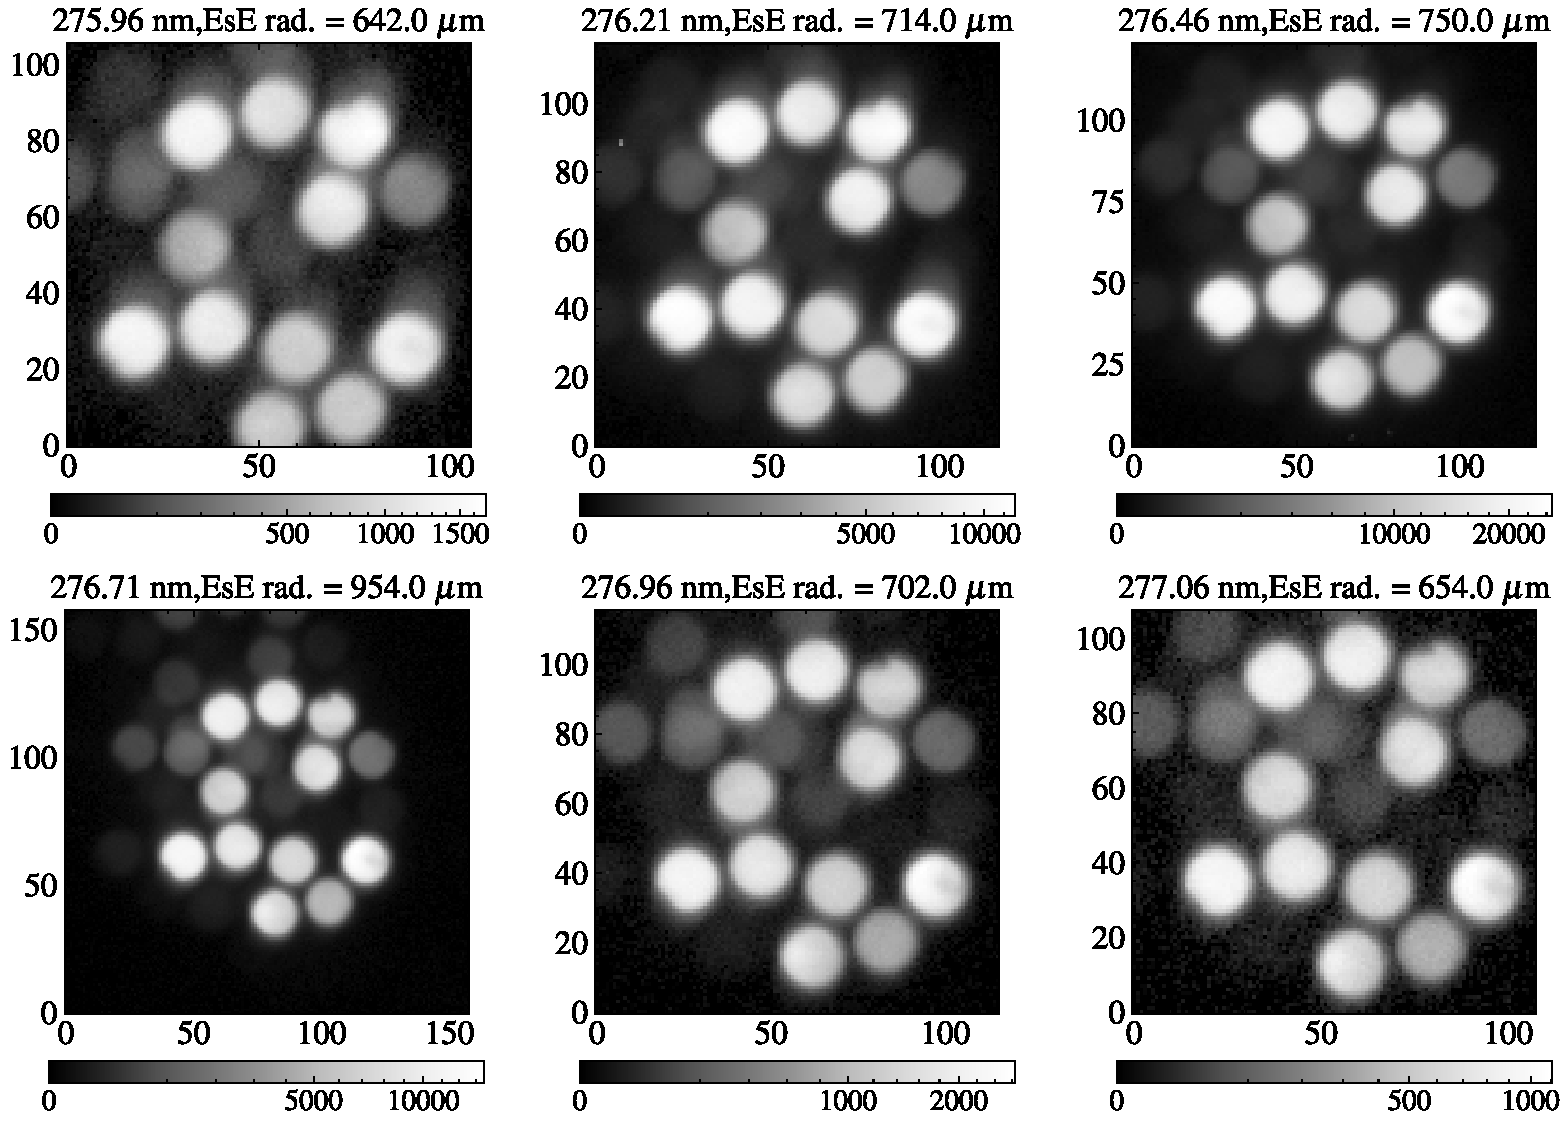
\includegraphics[trim={0cm 0cm 0cm 0cm},clip,width=0.9\linewidth]{nb2_images_edit.pdf}
\end{center}
\caption 
{\label{fig:nb2_images} Images captured at various wavelengths for the NB02 filter of \suit. The measurement wavelength and the 99\% ensquared energy radius are quoted at the top of each panel. The axes of the images are in units of image pixels.} 
\end{figure*}
%%%%%%%%%%%%%%%%%%%%%%%%%%%

%%%%%%%%%%%%%%%%%%%%%%%%%%%
\begin{figure*}
\begin{center}
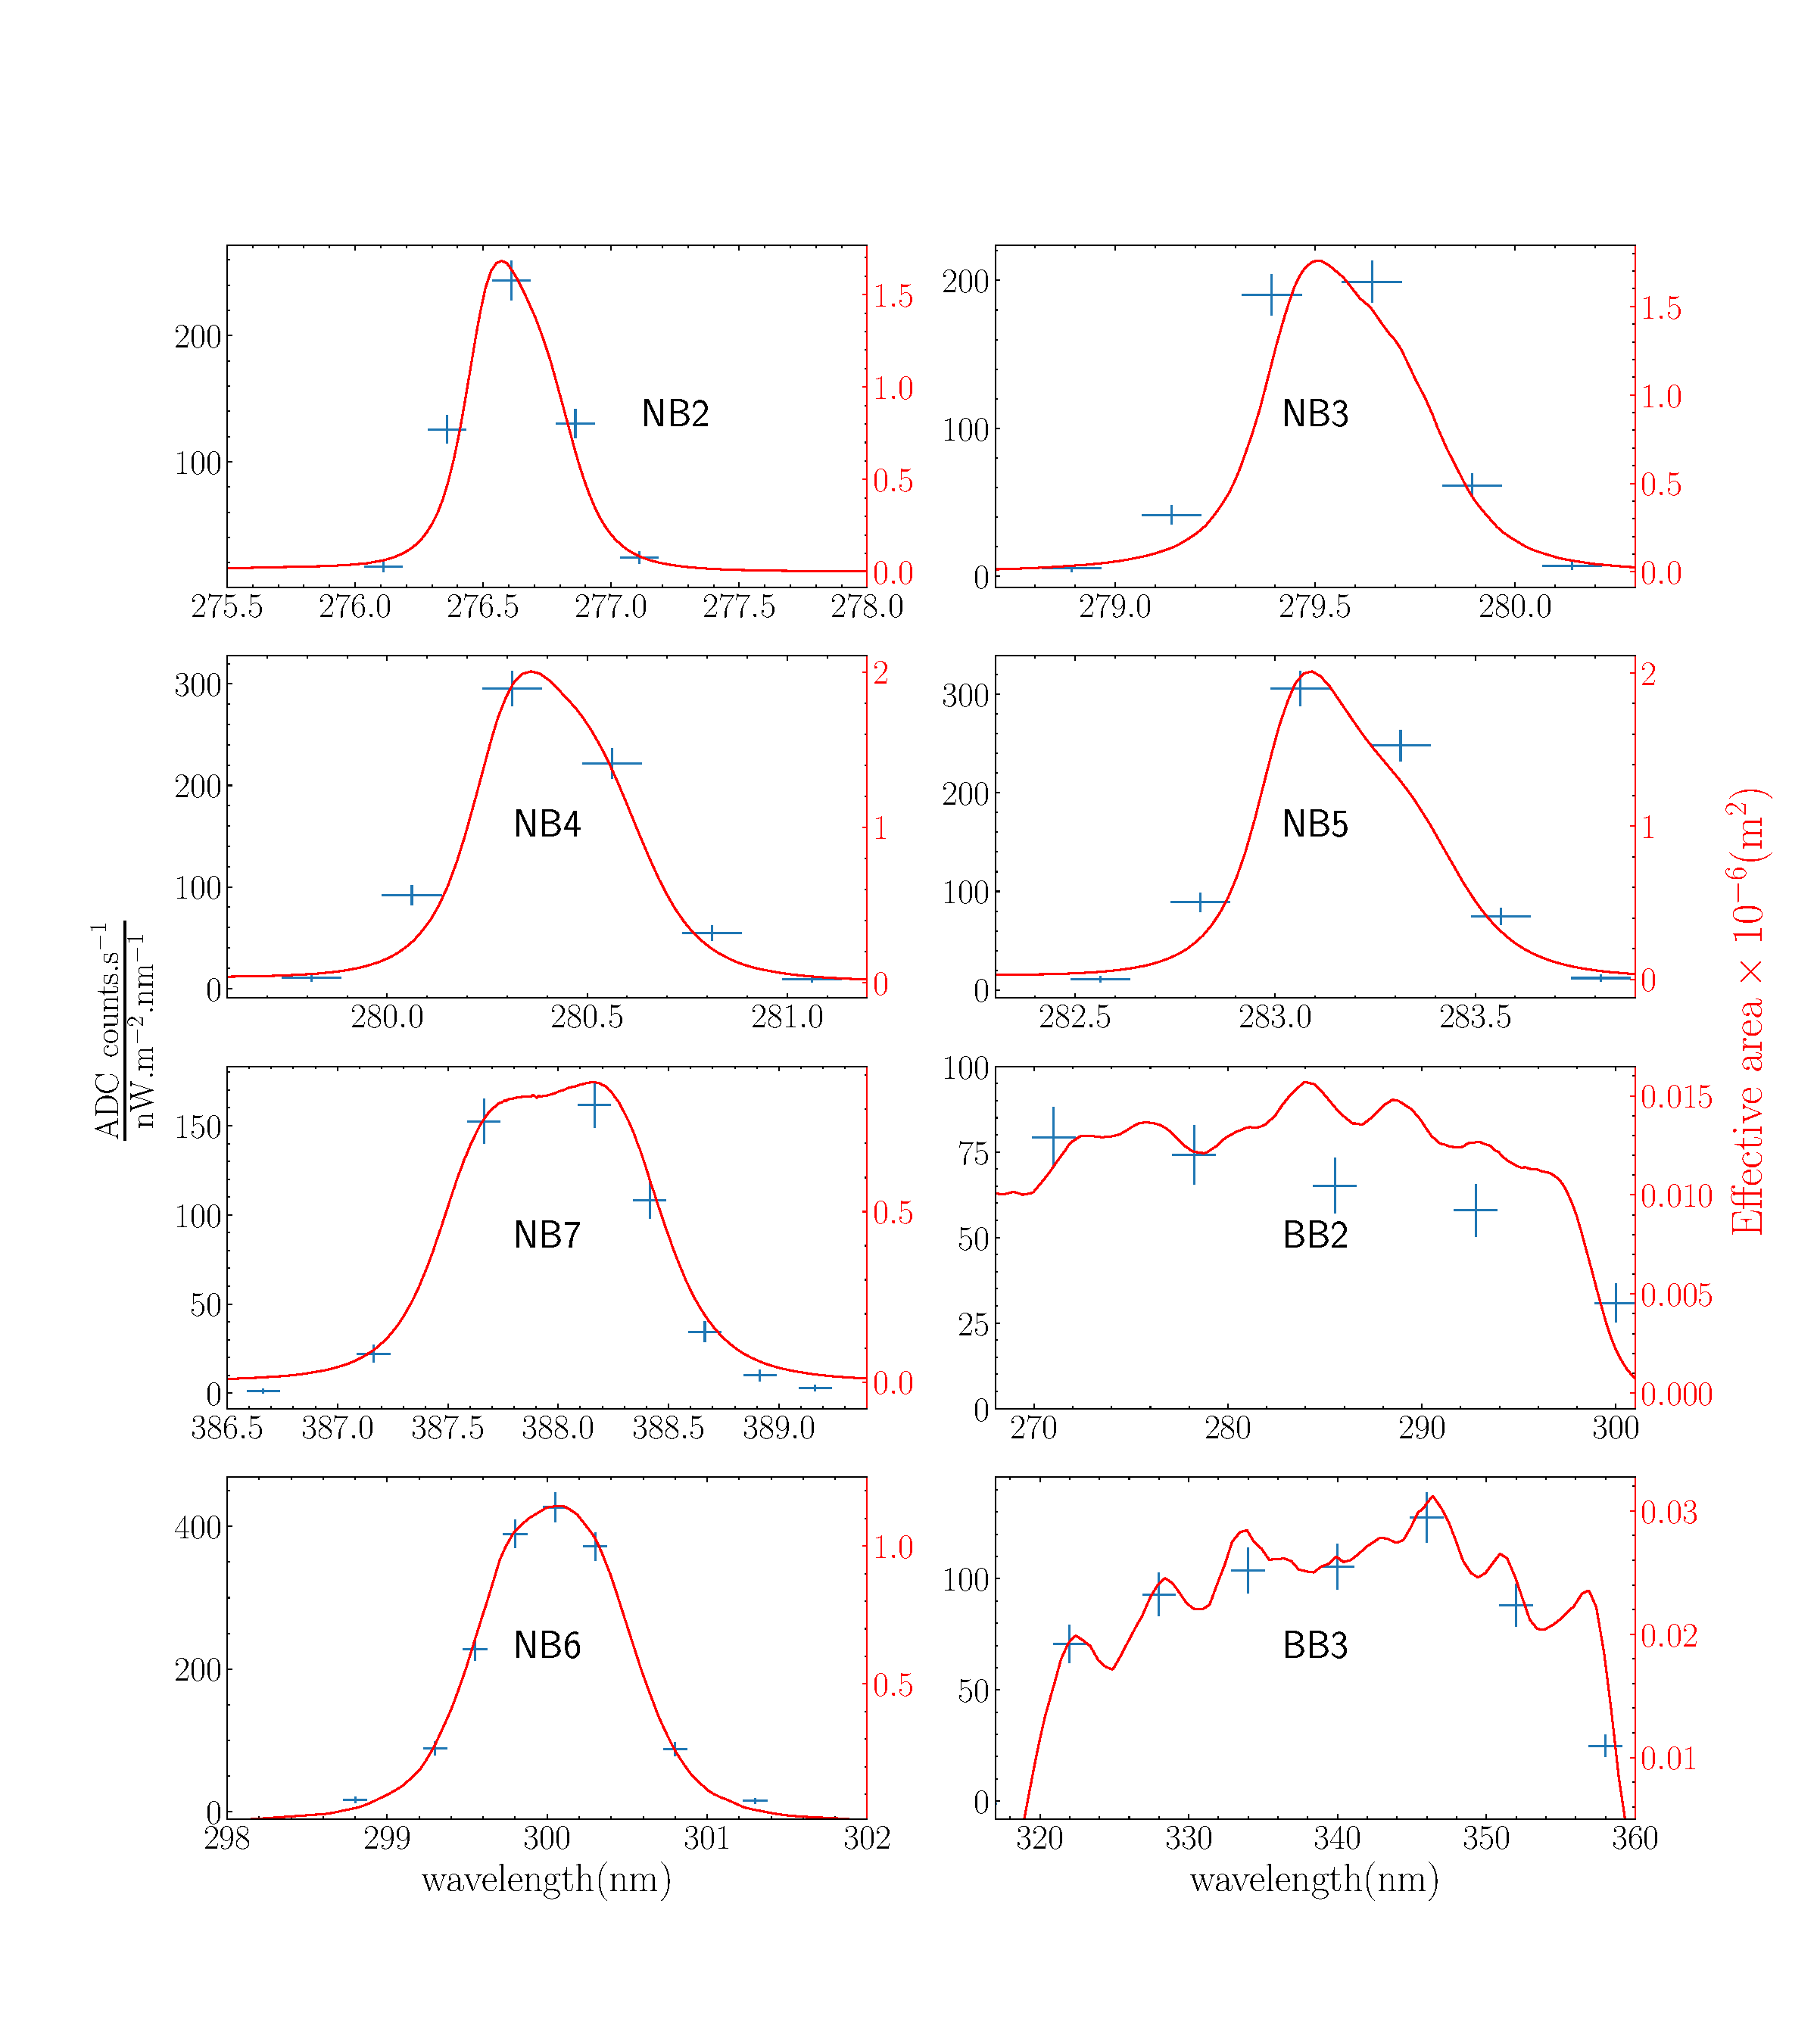
\includegraphics[trim={2.1cm 3.2cm 1.2cm 5.2cm},clip,width=0.95\textwidth] {spec_calib_new.pdf}
\end{center}
\caption 
{\label{fig:sepc_calib} Spectral validation for various filter combinations inferred from the imaging measurements (blue markers). The wavelength bins give the $x$ errors for the given input slit size. The Poisson uncertainty of the measured ADC counts gives the $y$ errors. The red solid curve shows the effective area calculated from measured transmission profiles of each component using Eqn \ref{eq:eff_area}.}
\end{figure*}
%%%%%%%%%%%%%%%%%%%%%%%%%%%

In Fig. \ref{fig:nb8_ghost} (a), we depict the fiber image captured at 396.85 nm. The position of the central image of the fiber, along with the sparsely spaced ghost reflections, is delineated by a white dashed box. Fig. \ref{fig:nb8_ghost} (b) offers a magnified perspective of this box, revealing the sparsely shaped ghost reflections indicated by white arrows. Some ghost reflections are observed very close to the central patch. Fig. \ref{fig:nb8_ghost} (c) provides a closer view around the central patch, with solid and dotted arrows indicating two closely spaced ghost reflections situated very close to the center. Given that these ghost reflections appear in proximity to the central patch and the relative brightness of the central patch to the ghost reflections fluctuates with wavelength, the estimation of the 99\% ensquared energy radius is also influenced.

%%%%%%%%%%%%%%
\begin{figure}
    \centering
    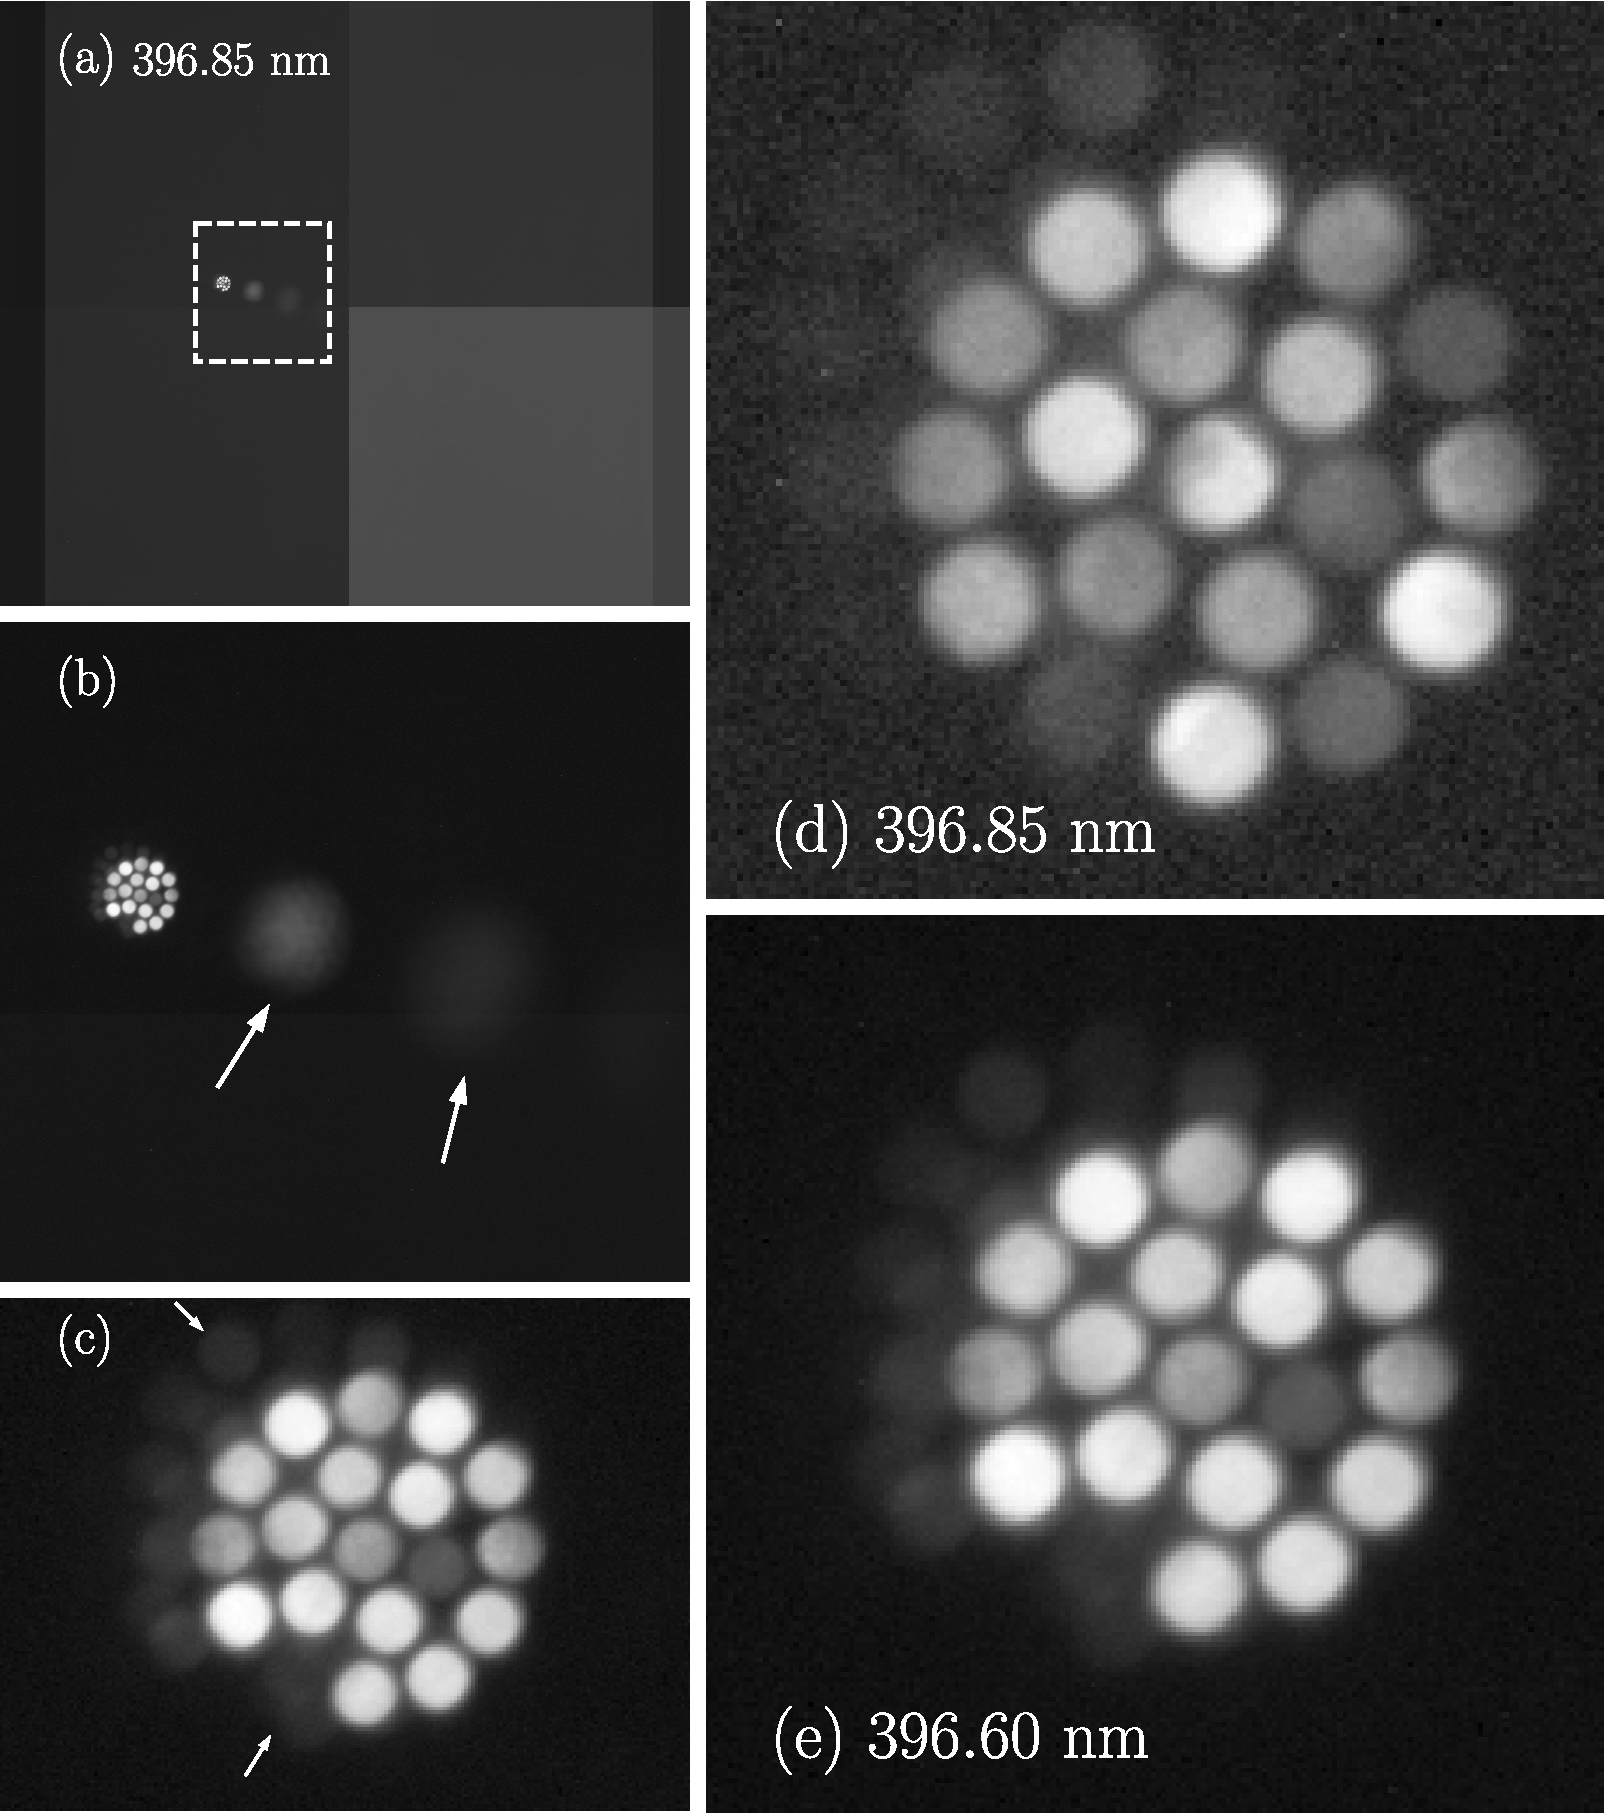
\includegraphics[width=0.8\textwidth]{nb8_ghost_im.pdf}
    \caption{(a) The ghost reflections of the optical fiber as seen with the NB08 filter. The input beam is centered at 396.85 nm. The position of the ghost reflections is marked with a white dashed box. (b) The zoomed-in view of the white dashed box. The arrows indicate sparsely spaced ghost reflections. (c) The arrows indicate two closely spaced ghost reflections close to the center. (d) 99\% ensquared energy box around the fiber bundle at 396.85 nm. (e) 99\% ensquared energy box around the fiber bundle at 396.60 nm.}
    \label{fig:nb8_ghost}
\end{figure}
%%%%%%%%%%%%%%

%%%%%%%%%%%%%%%%%%%%%%%%%%%%%%%%%%%%%%%%%%%%
\section{Stellar Calibration of  {\suit}}\label{sec:stellar_calib}
%%%%%%%%%%%%%%%%%%%%%%%%%%%%%%%%%%%%%%%%%%%%

The various science goals of \suit~were already mentioned in \S\ref{sec:suit}. To address these scientific objectives, the necessity of absolute stellar calibration is manifold. \suit, with its capabilities, will be imaging the Sun and dynamic processes such as solar flares and jets occurring in the solar atmosphere, including eruptions of various scales. Additionally, it will assist in measuring solar irradiance across 11 different passbands, probing various heights in the solar atmosphere from the photosphere to the chromosphere. With absolute calibration, we would be able to probe the underlying physical mechanisms driving these processes.

Many properties of white-light flares are also observable in the near-ultraviolet (NUV) regime. Typically, there are significant correlations between different flare quantities in white light and X-ray emissions, such as white-light excess and soft X-ray flux \citep{benz16,hudson16}. These correlations enable us to infer underlying mechanisms that likely drive the correlation between these quantities, such as the mechanisms responsible for transferring energy and mass across different layers of the Sun. In our case, \suit~would observe the Sun alongside HEL1OS and SoLEXS \citep{solexs}. For comparative purposes across observations from three different instruments, absolute calibration becomes essential.

Furthermore, in conjunction with \suit, the HEL1OS and SoLEXS data provide broad coverage of the electromagnetic spectrum from hard X-rays to the NUV. This comprehensive coverage allows us not only to study the initiation and triggering of eruptive events, but also to examine these quantities over a solar cycle and assess their contribution to changes in the solar spectral irradiance. Lastly, it's important to note that the Earth's atmosphere absorbs UV and X-ray emissions. UV radiation below 310 nm is largely absorbed by the atmosphere, while radiation beyond 310 nm can penetrate it. The absorption dynamics are primarily governed by oxygen ($O_{2}$) below 200 nm and ozone ($O_{3}$) beyond 240 nm, with both substances actively participating in the absorption process between 200 and 240 nm \citep{haigh07}. Therefore, understanding the solar spectral irradiance in the 200-400 nm range is pivotal for comprehending the dynamics and chemistry of Earth's atmosphere, particularly the ozone-oxygen cycle. This data serves as a crucial input for atmospheric modeling and provides insights into the Sun-Earth atmosphere connection. With absolute stellar calibration, \textit{SUIT} would furnish us with the solar irradiance in these bands and the radiance of various features on the solar disk before it encounters atmospheric attenuation.

\suit~is equipped with 16 LEDs, with 8 each operating at two distinct peak wavelengths: 258 nm and 356 nm, primarily for calibration purposes. However, it's worth noting that LEDs may degrade over time and do not offer fluxes corresponding to each individual filter. We have obtained measurements of flux-to-count ratio at various wavelengths within the extent of the science filter bands. This data will undoubtedly assist us in providing absolute calibration to \suit~observations. Nevertheless, unlike LEDs, while we can quantify how the overall throughput of the science filter combinations changes over time, we cannot quantify how the effective area of the science filter combination degrades as a function of wavelength. This degradation would impact the radiometric calibration using these measurements over time. Therefore, calibration through alternative methods is necessary, such as utilizing standard astronomical sources.

In an ideal scenario, the captured image would remain unaltered, devoid of any artifacts introduced by the instrumentation. However, in practice, the obtained image is influenced by the instrumental response, which can degrade over time. Radiometric calibration involves quantifying the instrumental response and using it to predict the actual signal received from the source.

Furthermore, \suit~ lacks in-band spectral resolution and lacks an accurate on-calibration lamp corresponding to the wavelength coverage of each individual filter. Therefore, it becomes imperative to convert the total in-band photo-electron count to the corresponding energy in real units. This necessity arises from the fact that photons across a wide band possess varying energy levels, making it challenging, if not impossible, to ascertain the distribution of photo-electrons across a band observation. Failure to address this adequately may impede our ability to effectively achieve one or more science goals of \suit.

In principle, for any astronomical source we encounter,

%------------------------------------------------------------
\begin{equation*}
    S(\lambda) = R(\lambda) \times F(\lambda);
\end{equation*}
%------------------------------------------------------------

where $F(\lambda)$, $S(\lambda)$ and $R(\lambda)$ are the emitted flux, measured signal and the response of the system at the wavelength $\lambda$, respectively. Here $R(\lambda)$ (instrumental response) will consists of the response from all the components of the telescope, namely thermal filter, the primary and secondary mirrors, science filter in conjunction with bandpass filer, focusing lens and the QE of the detector (a CCD in this case). In the case of an standard source we can write,

%------------------------------------------------------------
\begin{equation*}
    S(\lambda)_{calib} = R(\lambda)_{calib} \times F(\lambda)_{calib},
\end{equation*}
%------------------------------------------------------------
\noindent Therefore,
%------------------------------------------------------------
\begin{equation*}
    R(\lambda)_{calib} = \frac{S(\lambda)_{calib}}{F(\lambda)_{calib}},
\end{equation*}
%------------------------------------------------------------

\noindent where the subscript `calib' denotes all variables related to the standard absolute calibration source. The parameter $R(\lambda)_{calib}$ represents a calibration factor acquired by observing a standard source using an instrument. Photon flux can be straightforwardly computed from an absolutely calibrated spectrum $F(\lambda)$ using the formula $PF(\lambda) = SF(\lambda) \times \frac{\lambda}{hc}$.

Similarly, for the target source under observation, we have,

%------------------------------------------------------------
\begin{equation*}
    S(\lambda)_{target} = R(\lambda)_{target} \times F(\lambda)_{target}
\end{equation*}

\noindent and 
\begin{equation}
    F(\lambda)_{target} = \frac{S(\lambda)_{target}}{R(\lambda)_{calib}}
\end{equation}
%------------------------------------------------------------
where, it is assumed that the instrumental response remains unchanged from the calibrated source to the target source being observed, and hence $R(\lambda)_{target}=R(\lambda)_{calib}$.

%------------------------------------------------------------
\subsection{Requirements of the calibration source} \label{req}
%------------------------------------------------------------

In general, for radiometric calibration, on-board standard sources such as diodes, LEDs, etc., or astronomical sources like standard stars are employed. However, in a space-based mission, the on-board artificial sources themselves undergo significant degradation, which needs to be meticulously modeled. Therefore, it is preferable to utilize standard stars as calibration sources, provided they satisfy the essential conditions listed below \citep{article2}.

%%%%%%%%%%%%%%%
\begin{itemize}
    \item The calibration source must exhibit adequate brightness within the wavelength region of interest, which spans from 200 to 400 nm in the current context, to achieve the requisite photometric accuracy across all science filters. In our case, the thermal filter at the entrance aperture significantly attenuates in-band solar flux (along with nearly all out-band flux) reaching the detector to prevent pixel saturation. This mechanism applies equally to the calibration sources. Hence, the calibration source must possess sufficient brightness to attain an acceptable signal-to-noise ratio (SNR) within a reasonable observation time.
    \item Ideally, the standard calibration source should exhibit minimal variability, with any changes occurring over timescales significantly longer than the time required to accumulate a sufficient number of photons from the source to achieve the desired level of photometric accuracy.
    \item  Preferably, the calibration source should not be integrated into a complex system. However, if it is, any accompanying components should be sufficiently weak so that the photon flux from them does not significantly contribute to the total flux of the system. Otherwise, it would be necessary to model the contribution of the companion(s) separately.
\end{itemize}
%%%%%%%%%%%%%%%

Any astronomical source that meets these criteria and has its spectral energy distribution (SED) studied and calibrated to absolute units would be suitable for radiometric calibration. Stars such as Sirius A (HD48915/HR2491) and Vega (HR7001) largely fulfill the aforementioned criteria, with the exception of Sirius A, which has a white dwarf companion known as Sirius B. However, the apparent magnitudes of Sirius A and Sirius B are $-1.46$ \citep{hoffleit91} and $8.44$ \citep{mccook99,holberg13} respectively, ensuring that the contribution from Sirius B is mostly negligible. The absolute calibrated spectra for both stars are depicted in Fig.~\ref{fig:spec_1} and are sourced from the CALSPEC archive, which contains composite stellar spectra used as flux standards in the Hubble Space Telescope (HST) system.

%------------------------------------------------------------
\begin{figure}
    \centering
    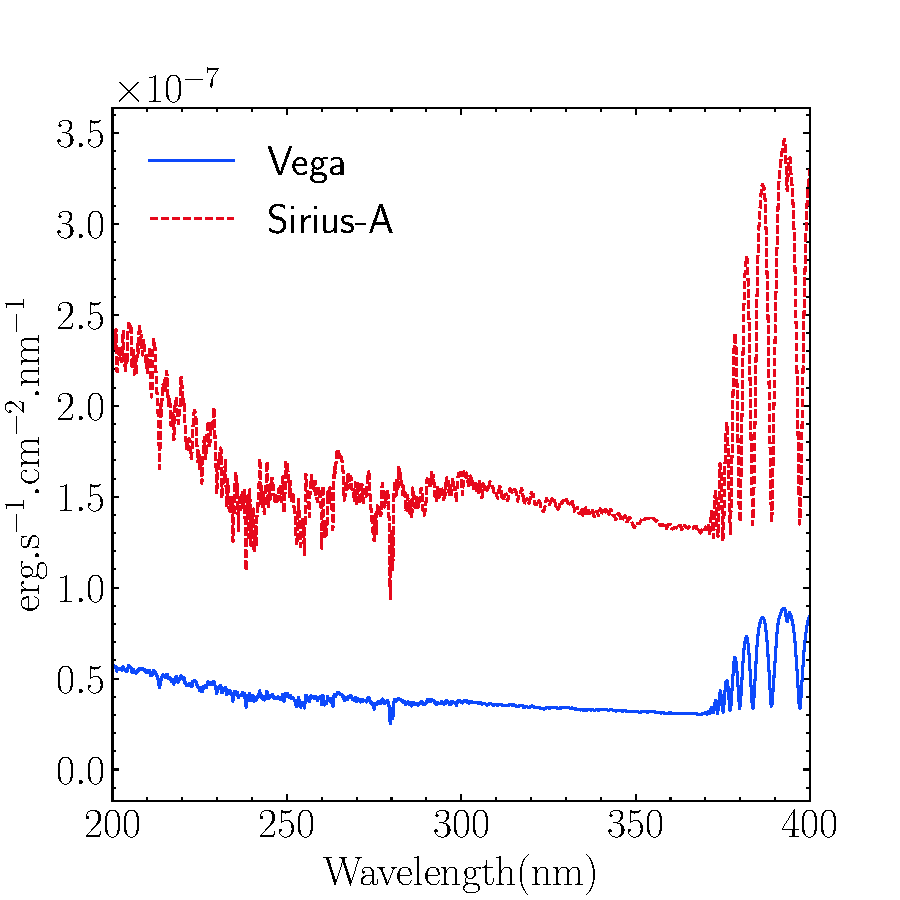
\includegraphics[width=0.7\linewidth]{spectrum_sir_veg.pdf}
    \caption{Calibrated spectra of Vega and Sirius A taken from \href{https://www.stsci.edu/hst/instrumentation/reference-data-for-calibration-and-tools/astronomical-catalogs/calspec}{CALSPEC}, Vega in Blue and Sirius A in Orange.}
    \label{fig:spec_1}
\end{figure}
%------------------------------------------------------------

%------------------------------------------------------------
\subsection{Exposure time for the calibration sources}\label{expo_time}
%------------------------------------------------------------

A high level of photometric accuracy is essential for imaging the Sun and monitoring spectral irradiance. It's noteworthy that the total energy output from the Sun at wavelengths below 400 nm comprises only about 8\% of the total solar irradiance (TSI). However, there is a recorded variability of over 60\% in radiation below 400 nm over a solar cycle \citep{krivova06}, whereas the variability in TSI over a solar cycle is approximately 0.1\%. Photometric accuracy is defined as the ratio of the Poisson noise of the signal to the signal itself. The number of photo-electrons produced in a given exposure time is give by Eqn.~\ref{eq1},\ref{eq:eff_area}. We aim for a photometric accuracy of 0.2\%, which corresponds to a photo-electron count of $\sim 2.5 \times 10^{5}$. Considering this requirement, we compute the exposure times required for both Vega and Sirius A, which are given in Table~\ref{tab_2}.

%-------------------------------------------------
\begin{table}
\centering
\begin{tabular}{ccccc}
\hline
        & Exposure time(minutes) & Exposure time(minutes) \\
        Band & Vega & Sirius A\\
        \hline
        NB1 & 8 & 2\\
        NB2 & 23 & 6\\
        NB3 & 23 & 6\\
        NB4 & 19 & 5\\
        NB5 & 16.5 & 4\\
        NB6 & 15 & 3.5\\
        NB7 & 12 & 3\\
        NB8 & 368 & 90\\
        BB1 & 2 & 0.5\\
        BB2 & 20 & 5\\
        BB3 & 13 & 3\\
        \hline
    \end{tabular}
    \caption{The exposure time required to obtain $2.5 \times 10^{5}$ photo-electrons to achieve 0.2\% photometric accuracy in each of the science filters for both Vega and Sirius A.}
\label{tab_2}
\end{table}

%%%%%%%%%%%%%%%%%%%%%%%%%%%%%%%%%%%%%%%%%%%%%%%%%%%%%%%%%
\subsection{Method for Calibration}\label{cal_meth}
%%%%%%%%%%%%%%%%%%%%%%%%%%%%%%%%%%%%%%%%%%%%%%%%%%%%%%%%%

With the exposure times calculated for all filters, for calibration purposes, we will assume a photometric accuracy of 0.2\% across all bands for the calibration source. This implies that the Poisson noise arising from the total photo electron count is 0.2\%, corresponding to a total photo electron count of approximately $2.5 \times 10^{5}$. As described in Section \ref{sec:stellar_calib}, the flux from the target source is given by $F(\lambda)_{\text{target}}=\frac{S(\lambda)_{\text{target}}}{R(\lambda)_{\text{calib}}}$, where we assume that the instrumental response $R(\lambda)_{\text{calib}}$ remains unchanged from the calibration source to the target source. Therefore, given a calibration source using the absolute spectra ($F(\lambda)_{\text{calib}}$) and the signal ($S(\lambda)_{\text{calib}}$) received from it, we can quantify the filter profiles ($R(\lambda)_{\text{calib}}$).

In the case of \suit, though there is no spectral resolution within the bands, and the only information we will obtain from an observation is the total number of photo electron counts from the bands for a given exposure time. The general method is as follows:

\begin{itemize}
    \item Given the spectra of a calibration source one can create the photo elctron count profiles using the instrument filter profiles.
    
    \item One can calculate the total number of photo elctrons generated for some exposure time as:
    \begin{equation*}
        DN_{calib} = \int P(\lambda)_{calib\hspace{0.1cm}}R(\lambda)\hspace{0.1cm}A\hspace{0.1cm}t\hspace{0.1cm} d\lambda
    \end{equation*}
    \noindent where, $P(\lambda)$ is the photon flux from the Calibration source.
    
    \item The inband energy from the spectra of the calibration source for the same exposure time can be calculated. The FWHM is taken to be the extent of each band while calculating the total energy.
    \begin{equation*}
        T_{calib} = \int_{inband} F(\lambda)_{calib}\hspace{0.1cm} A\hspace{0.1cm}t\hspace{0.1cm} d\lambda
    \end{equation*}
    \item The ratio of these two quantities give the calibration constant, `C' for each band, C = $\frac{T_{calib}}{DN_{calib}}$
\end{itemize}

To estimate how well this method performs, we use Vega (Sirius~A) as the calibration source and produce the phtoelctron count profiles from Sirius~A (Vega) and the Sun. The total count arising from each band multiplied by the calibration constant(C) should give the total energy from the spectra.

%------------------------------------------------------------
\subsection{Sirius A as calibration source}\label{sirius}
%------------------------------------------------------------

Table~\ref{tab:my_table_sun_sir} shows the performance of the method for a Sirius A as the calibrating source and sun as a target with 200s exposure in all bands. The uncertainties in the table~\ref{tab:my_table_sun_sir} are obtained by propagating the uncertainties of the \href{https://www.stsci.edu/hst/instrumentation/reference-data-for-calibration-and-tools/astronomical-catalogs/calspec}{CALSPEC} spectra. Key thing to note here, the comparisons for Solar spectra are made with a sun as a star spectra, while SUIT is going to observe the full solar disk on $(4k \times 4k)$ CCD. We have to add the contribution from all the pixels to have the full disk contribution. In practice, in the stellar pointing calibration run \suit~will be re-pointed towards Sirius A and the measurements would be used for absolute calibration.

%------------------------------------------------------------
\begin{table}[ht!]
\small
\centering
    \begin{tabular}{|ccccc|}
    \hline
        Band & $(C=\frac{T_{sir}}{DN_{sir}})\times 10^{15}$ & DN/$10^{13}$ & Predicted Energy & Energy from \\
         & (J/DN) & & ($C \times DN$) & spectra(J) \\
        \hline
        \hline
        NB1 & $(72.62\pm0.88)$ & $(9.47 \pm 9.7 \times 10^{-7})$ & $(6.881 \pm 0.083)$ & 6.839\\
        \hline
        NB2 & $(5.164\pm0.062)$ & $(20.6\pm1.4\times10^{-6})$ & $(1.065\pm0.013)$ & $1.072$\\
        \hline
        NB3 & $(3.627\pm0.044)$ & $(10.5\pm1.0\times10^{-6})$ & $(3.854\pm0.043)\times10^{-1}$ & $3.884\times10^{-1}$ \\
        \hline
        NB4 & $(3.253\pm0.039)$ & $(12.3\pm1.1\times10^{-6})$ & $(4.003\pm0.048)\times10^{-1}$ & $(4.001\times10^{-1})$ \\
        \hline
        NB5 & $(3.160\pm0.038)$ & $(40.6\pm2.0\times10^{-6})$ & $(1.284\pm0.016)$ & $1.307$ \\
        \hline
        NB6 & $(7.295\pm0.088)$ & $(65.7 \pm 2.6 \times 10^{-6})$ & $(4.797\pm0.058)$ & $4.836$ \\
        \hline
        NB7 & $(8.715\pm0.010)$ & $(123 \pm 4 \times 10^{-6})$ & $(1.073\pm0.013)\times10^{1}$ & $1.055\times10^{1}$ \\
        \hline
        NB8 & $(17.71\pm0.21)$ & $(5.01 \pm 7.1 \times 10^{-7})$ & $(8.88\pm0.11)\times10^{-1}$ & $8.93\times10^{-1}$ \\
        \hline
        BB1 & $(28.50\pm0.41)$ & $(46.0 \pm 2.1 \times 10^{-6})$ & $(13.114\pm0.188)$ & 13.113 \\
        \hline
        BB2 & $(469.9\pm5.7)$ &$(28.3 \pm 1.7 \times 10^{-6})$ & $(132.997\pm1.607)$ & 132.994 \\
        \hline
        BB3 & $(221.1\pm2.7)$ & $(176 \pm 4 \times 10^{-6})$ & $(3.903\pm0.047)\times10^{2}$ & $3.896\times10^{2}$\\
        \hline
    \end{tabular}
    \caption{The performance of the method with Sirius A as calibrating source and sun as a target with 200s exposure in all bands.}
\label{tab:my_table_sun_sir}
\end{table}
%------------------------------------------------------------


%%%%%%%%%%%%%%%%%%%%%%%%%%%%%%%%%%%%%%%%%%%%
%\section{Filter Choice for {\suit}}\label{sec:suit_filter_choice}
%%%%%%%%%%%%%%%%%%%%%%%%%%%%%%%%%%%%%%%%%%%%

%%%%%%%%%%%%%%%%%%%%%%%%%%%%%%%%%%%%%%%%%%%%
\section{Outlook}\label{sec:c3_outlook}
%%%%%%%%%%%%%%%%%%%%%%%%%%%%%%%%%%%%%%%%%%%%

\suit~is our first full-disk eye on the Sun in \ion{Mg}{2} window and \ion{Ca}{2} h line \sr{is this technically true? SOT did observe in the same wavelength. How much of it was full-disk?} and the various continuum channels onboard. The narrow band continuum and line channels provide us with targeted view into various layers of the sun, while the three broad band channels are designed to probe the radiance from the Sun, to investigate the effect on Earth's atmosphere over the duration of a solar cycle. This chapter focused on the various initial preparatory analysis we carried out in anticipation of \suit, and some of the calibration scheme planning initially carried on.

The initial jitter estimation was done from simulations provided by the ISRO URSC team. That exhibited the jitter to be minimal compared to \suit~exposure timescales, hence would have no noticeable effects on the imaging. The proper estimation of the spacecraft jitter on orbit would be possible once the stellar calibration is done. During the stellar calibration the long exposure of Sirius-A, {\it i.e.} a point source would be carried out in a series of short exposures. This would give us the opportunity to quantify the amount of jitter of the spacecraft.

The initial throughput model of \suit~was designed out of the necessity of a robust throughput model to estimate the expected SNR of various vendor provided science filters, in accordance to the scientific cases. It proved useful in finalizing the choice of the science filters to be mounted on the the payload. The throughput model also proved useful in designing our stellar calibration scheme, and provided a useful benchmark for validating the photometric performance of the payload on ground. The spectral validation of the science filters is important primarily for verifying the science filter combinations are observing the necessary wavelength windows. The necessity of a accurate throughput model, spectral and photometric validation of the payload, stellar calibration of the payload are intertwined with one another. A full characterization of all of these quantities is only possible after steallr callibration is carried out. 